\documentclass[UTF8]{ctexrep} % Chinese language class type, need XeLaTeX to compile
\usepackage{hologo} % needed for reference
\usepackage{gbt7714} % needed for reference
\usepackage{float} % needed for [H] strick floating option
\usepackage{caption} % needed for command \captionsetup in longlisting new environment
\usepackage{subcaption} % needed for command \captionsetup in longlisting new environment
\usepackage{graphicx} % needed for displaying eps file
\usepackage{longtable} % to display tables on several pages
\usepackage{rotating} % to display tables in landscape
\usepackage{multirow} % for multirow tables
\usepackage{booktabs} % for prettier tables
\usepackage[title]{appendix} % create appendices
%-----------------------------------------------------------------------------------------
% To write pseudo-code
%-----------------------------------------------------------------------------------------
\usepackage{algorithm}  
\usepackage{algpseudocode}
\usepackage{amsmath}
\usepackage{amssymb}
\renewcommand{\algorithmicrequire}{\textbf{Input:}}  % Use Input in the format of Algorithm  
\renewcommand{\algorithmicensure}{\textbf{Output:}} % Use Output in the format of Algorithm
%-----------------------------------------------------------------------------------------
% To adjust geometry and stuff
%-----------------------------------------------------------------------------------------
\usepackage{geometry} % adjust margin and what
\geometry{a4paper} % use A4 paper to make the report look good enough
%-----------------------------------------------------------------------------------------
% To define colors yourself
%-----------------------------------------------------------------------------------------
\usepackage{xcolor} % needed for defining own color
% \definecolor{myred}{RGB}{223, 56, 27}
% \definecolor{myblue}{RGB}{25, 123, 193}
% \definecolor{myorange}{RGB}{225, 107, 65}
% \definecolor{mypink}{RGB}{254, 63, 125}
% \definecolor{mycyan}{RGB}{72, 199, 240}
% \definecolor{mygreen}{RGB}{0, 153, 136}
%-----------------------------------------------------------------------------------------
% To use hyper-reference and stuff
%------- ----------------------------------------------------------------------------------
\usepackage{hyperref} % needed for hyperlinks
\hypersetup{ % hyper link setups, can be used else where
    colorlinks=true,
    linkcolor=blue,
    filecolor=magenta,      
    urlcolor=cyan,
    pdftitle={miniSQL},
}
%-----------------------------------------------------------------------------------------
% To list code elegantly and stuff
%-----------------------------------------------------------------------------------------
\usepackage[
    % cache=false,
    newfloat=true,
    % outputdir=./
]{minted} % needed for listing
\newenvironment{longlisting}{\captionsetup{type=listing}}{}
\setminted{
    tabsize=4,
    breaklines,
    frame=single,
    linenos,
    fontsize=\small
}
% \usepackage{bold-extra}
% \usepackage[T1]{fontenc}
% \usepackage{libertine} % this is a temp solution, should consider on using other packages for font
\makeatletter
\newenvironment{breakablealgorithm}
  {% \begin{breakablealgorithm}
   \begin{center}
     \refstepcounter{algorithm}% New algorithm
     \hrule height.8pt depth0pt \kern2pt% \@fs@pre for \@fs@ruled
     \renewcommand{\caption}[2][\relax]{% Make a new \caption
       {\raggedright\textbf{\ALG@name~\thealgorithm} ##2\par}%
       \ifx\relax##1\relax % #1 is \relax
         \addcontentsline{loa}{algorithm}{\protect\numberline{\thealgorithm}##2}%
       \else % #1 is not \relax
         \addcontentsline{loa}{algorithm}{\protect\numberline{\thealgorithm}##1}%
       \fi
       \kern2pt\hrule\kern2pt
     }
  }{% \end{breakablealgorithm}
     \kern2pt\hrule\relax% \@fs@post for \@fs@ruled
   \end{center}
  }
\makeatother

% \algrenewtext{For}[3]%
% {\algorithmicfor\ #1 \gets #2 \algorithmicto\ #3 \algorithmicdo}


%-----------------------------------------------------------------------------------------
% To predefine title and stuff
%-----------------------------------------------------------------------------------------
\begin{document}

\begin{titlepage}
	\centering
	
\includegraphics[width=0.75\textwidth]{figure/浙江大学.eps}\par\vspace{1cm}
% 	{\scshape\LARGE Columbidae University \par}
% 	\vspace{1cm}
	{\scshape\LARGE 数据库系统实验报告\par}
	\vspace{1.5cm}
	{\huge\textsc{\textsc{miniSQL}}\textbf{小组实验报告}\par}
	\vspace{2cm}
	{\Large\itshape 徐\ \ 震 \textbf{3180105504} 18888916826\par}
	{\Large\itshape 曾一欣 \textbf{3180105144} 13372553368\par}
	{\Large\itshape 毛一恒 \textbf{3180103727} 13587492148\par}
	\vfill
	指导教师\par
	\textit{孙建伶}

	\vfill

% Bottom of the page
	{\large \today\par}
\end{titlepage}


\newpage
\tableofcontents
\newpage
\part{正文}
\chapter{实验目的}
\section{总体实验目的}
\subsection{\textsc{miniSQL}}
设计并实现一个精简型单用户SQL引擎(DBMS)\textsc{miniSQL},允许用户通过字符界面输入SQL 语句实现表的建立/删除;索引的建立/删除以及表记录的插入/删除/查找。

\subsection{设计目的}
通过对\textsc{miniSQL}的设计与实现,提高学生的系统编程能力,加深对数据库系统原理的理解。
通过编程设计,加深对数据库系统的理解并深入了解B+树这一数据结构。
以模块化方式构建大型计算机软件,提高架构抽象能力并重视模块化和解耦合在软件设计中的作用。

\section{模块实验目的}
\subsection{索引管理器}
我们负责设计的索引管理器模块主要负责数据库系统中的索引管理,提供基于B+树的索引实现并提高数据库查询/插入/删除效率。并通过提供易用接口与其他模块整合实现有效功能。

\subsection{缓存管理器}
负责缓冲区的管理,主要功能有:
1. 根据需要,读取指定的数据到系统缓冲区或将缓冲区中的数据写出到文件。
2. 实现缓冲区的替换算法,当缓冲区满时选择合适的页进行替换。
3. 记录缓冲区中各页的状态,如是否被修改过等。
4. 提供缓冲区页的pin功能,及锁定缓冲区的页,不允许替换出去。

\subsection{记录管理器}
负责管理记录表中数据的数据文件。主要功能为实现数据文件的创建与删除(由表的定义与删除引起)、记录的插入、删除与查找操作,并对外提供相应的接口。其中记录的查找操作要求能够支持不带条件的查找和带一个条件的查找(包括等值查找、不等值查找和区间查找)。数据文件由一个或多个数据块组成,块大小应与缓冲区块大小相同。一个块中包含一条至多条记录,为简单起见,只要求支持定长记录的存储,且不要求支持记录的跨块存储。

\subsection{目录管理器}
负责管理数据库的所有模式信息,包括:
1. 数据库中所有表的定义信息。
2. 表中每个字段的定义信息。
3. 数据库中所有索引的定义。

\subsection{接口管理器}
接口管理器模块是整个系统的核心,其主要功能为提供执行SQL 语句的接口,解释器层调用。解释器 层解释生成的命令内部表示为输入,根据目录管理器提供的信息确定执行规则,并调用记录管理器去,索引管理器,目录管理器提供的相应接口进行执行,最后返回执行结果给解释器模块。

\subsection{命令行解释器}
解释器模块直接与用户交互,主要实现以下功能:
1. 程序流程控制,即“启动并初始化→‘接收命令、处理命令、显示命令结果’循环→退出”流程。
2. 接收并解释用户输入的命令,生成命令的内部数据结构表示,同时检查命令的语法正确性和部分语义正确性,对正确
的命令调用API 层提供的函数执行并显示执行结果,对不正确的命令显示错误信息。

\subsection{图形界面}
我们通过实现图形界面以环节用户对于命令行界面的恐惧(纵使这个图形界面中用户还是要敲写SQL语句),通过\texttt{PyQt}等易用接口实现一个简单的带有语法高亮的编辑器界面,并用对用户友好的方式输入输出各种信息,并提供对于一般编辑器操作的支持(例如多种快捷键和其他功能)。

\chapter{系统需求}
\section{需求概述}
\subsection{数据类型}
只要求支持三种基本数据类型:int,char(n),float,其中char(n)满足 1 <= n <= 255 。
\subsection{表定义}
一个表最多可以定义32 个属性,各属性可以指定是否为unique;支持unique 属性的主键定义。
\subsection{索引的建立和删除}
对于表的主键自动建立B+树索引,对于声明为unique 的属性可以通过SQL 语句由用户指定建立/删除B+树索引(因此,所
有的B+树索引都是单属性单值的)。
\subsection{查找记录}
可以通过指定用and 连接的多个条件进行查询,支持等值查询和区间查询。
\subsection{插入和删除记录}
支持每次一条记录的插入操作;
支持每次一条或多条记录的删除操作。(where 条件是范围时删除多条)

\section{语法说明}
\textsc{miniSQL}支持标准的SQL语句格式,每一条SQL 语句以分号结尾,一条SQL 语句可写在一行或多行。为简化编程,要求所有的关键字都为小写。在以下语句的语法说明中,用黑体显示的部分表示语句中的原始字符串,如\textbf{create}就严格的表示字符串“create”,其他非黑体显示的有其他的含义,如 表名 并不是表示字符串 “表名”,而是表示表的名称。
\subsection{创建表语句}
该语句的语法如下:
\begin{longlisting}
    \begin{minted}{mysql}
-- 语法说明
create table 表名 (
    列名 类型 ,
    列名 类型 ,
    列名 类型 ,
    primary key ( 列名 )
);

-- 示例
create table student (
    sno char(8),
    sname char(16) unique,
    sage int,
    sgender char (1),
    primary key ( sno )
);
    \end{minted}
    \caption{Create Table Syntax and Example}
    \label{lst:create_table_requirements}
\end{longlisting}
其中类型的说明见第二节“功能需求”。
若该语句执行成功,则输出执行成功信息;若失败,必须告诉用户失败的原因。

\subsection{删除表语句}
该语句的语法如下:
若该语句执行成功,则输出执行成功信息;若失败,必须告诉用户失败的原因。
\begin{longlisting}
    \begin{minted}{mysql}
-- 语法说明
drop table 表名 ;
-- 示例语句:
drop table student;
    \end{minted}
    \caption{Drop Table Syntax and Example}
    \label{lst:drop_table_requirements}
\end{longlisting}

\subsection{创建索引语句}
该语句的语法如下:
若该语句执行成功,则输出执行成功信息;若失败,必须告诉用户失败的原因。
\begin{longlisting}
    \begin{minted}{mysql}
-- 语法说明
create index 索引名 on 表名 ( 列名 );
-- 示例语句:
create index stunameidx on student ( sname );
    \end{minted}
    \caption{Create Index Syntax and Example}
    \label{lst:create_index_requirements}
\end{longlisting}

\subsection{删除索引语句}
该语句的语法如下:
若该语句执行成功,则输出执行成功信息;若失败,必须告诉用户失败的原因。
\begin{longlisting}
    \begin{minted}{mysql}
-- 语法说明
drop index 索引名 ;
-- 示例语句
drop index stunameidx;
    \end{minted}
    \caption{Drop Index Syntax and Example}
    \label{lst:drop_index_requirements}
\end{longlisting}

\subsection{选择语句}
该语句的语法如下:
\begin{longlisting}
    \begin{minted}{mysql}
-- 语法说明
select * from 表名 ;
-- 或:
select * from 表名 where 条件 ;
-- 示例语句
select * from student;
select * from student where sno = '88888888';
select * from student where sage > 20 and sgender = 'F';
    \end{minted}
    \caption{Select Syntax and Example}
    \label{lst:select_requirements}
\end{longlisting}
其中“条件”具有以下格式:$列 op 值 and 列 op 值 … and 列 op 值$。
op 是算术比较符:$= <> < > <= >=$
若该语句执行成功且查询结果不为空,则按行输出查询结果,第一行为属性名,其余每一行表示一条记录;若查询结果为空,
则输出信息告诉用户查询结果为空;若失败,必须告诉用户失败的原因。

\subsection{插入记录语句}
该语句的语法如下:
若该语句执行成功,则输出执行成功信息;若失败,必须告诉用户失败的原因。
\begin{longlisting}
    \begin{minted}{mysql}
-- 语法说明
insert into 表名 values ( 值1 , 值2 , … , 值n );
-- 示例语句
insert into student values ('12345678','wy',22,'M');
    \end{minted}
    \caption{Insert Syntax and Example}
    \label{lst:insert_requirements}
\end{longlisting}

\subsection{删除记录语句}
该语句的语法如下:
\begin{longlisting}
    \begin{minted}{mysql}
-- 语法说明
delete from 表名 ;
-- 或:
delete from 表名 where 条件 ;
-- 示例语句
delete from student;
delete from student where sno = '88888888';
    \end{minted}
    \caption{Delete From Syntax and Example}
    \label{lst:delete_from_requirements}
\end{longlisting}
若该语句执行成功,则输出执行成功信息,其中包括删除的记录数;若失败,必须告诉用户失败的原因。

\subsection{退出\textsc{miniSQL}系统语句}
该语句的语法如下:
\begin{longlisting}
    \begin{minted}{mysql}
-- 语法说明
quit;
exit;
    \end{minted}
    \caption{Quit miniSQL Syntax}
    \label{lst:quit_miniSQL_requirements}
\end{longlisting}

\subsection{执行SQL脚本文件语句}
该语句的语法如下:
\begin{longlisting}
    \begin{minted}{mysql}
-- 语法说明
execfile 文件名 ;
    \end{minted}
    \caption{Execute File Syntax}
    \label{lst:execfile_requirements}
\end{longlisting}
SQL 脚本文件中可以包含任意多条上述8 种SQL 语句,MiniSQL 系统读入该文件,然后按序依次逐条执行脚本中的SQL
语句。

\subsection{关于返回信息}
返回信息的内容参考mysql,语言限定为英文,主要包括执行sql返回的行数(n row in set), 或者影响的行数(n row affects),
必须给出执行SQL所花费的时间Duration。
执行出错需要指出错误的类型,具体位置不做要求。
错误类型包括(SYNTAX ERROR, INVALID INDENTIFIER, INVALID VALUE , INVALID ATTR FOR INDEX),即语法错
误(语法参考mysql,miniSQL 不支持的数据类型和SQL 等也报语法错误), 标识符错误(不存在的表名,字段名等) , 值错误(变量
长度不足以容纳实际数据), 索引定义在非unique 属性上。
可以参考mysql workbench和mysql terminal client的返回信息。

\subsection{关于辅助性命令语句}
我们定义了如下的辅助性质语句来方便用户使用本数据库.
\begin{longlisting}
    \begin{minted}{mysql}
-- 语法说明
show tables;
show index from 表名;
show create table 表名;

-- 示例
show tables;
show index from student2;
show create table student2;
    \end{minted}
    \caption{辅助语句}
    \label{lst:auxiliary_syntax}
\end{longlisting}

\subsection{关于图形界面}
我们希望开发一个图形界面以管理用户的输入输出,提供基本按钮和快捷键。并提供图标等。
\begin{figure}[H]
    \centering
    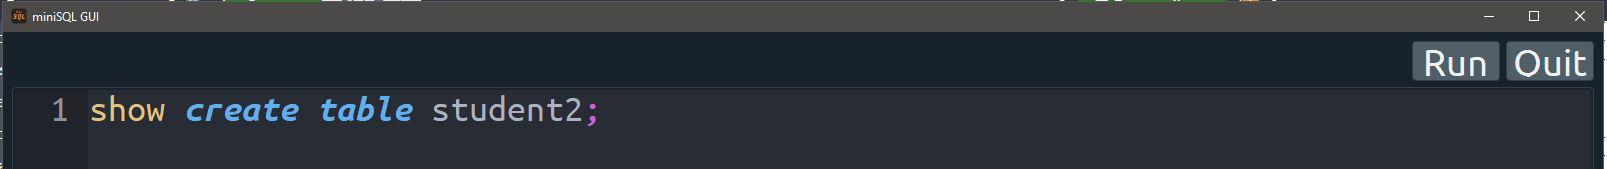
\includegraphics[width=\linewidth]{figure/gui_requirements.png}
    \caption{GUI Requirements}
    \label{fig:gui_requirements}
\end{figure}
\subsection{关于代码编辑器}
我们希望提供一个带有代码高亮功能,自动补全功能,自动换行功能,以及各种编辑器快捷键(复制一行,列操作,关键词操作)等的完整小型sql语句编辑视窗。
同时,我们希望\textsc{miniSQL}支持多行语句执行的操作。
\begin{figure}[H]
    \centering
    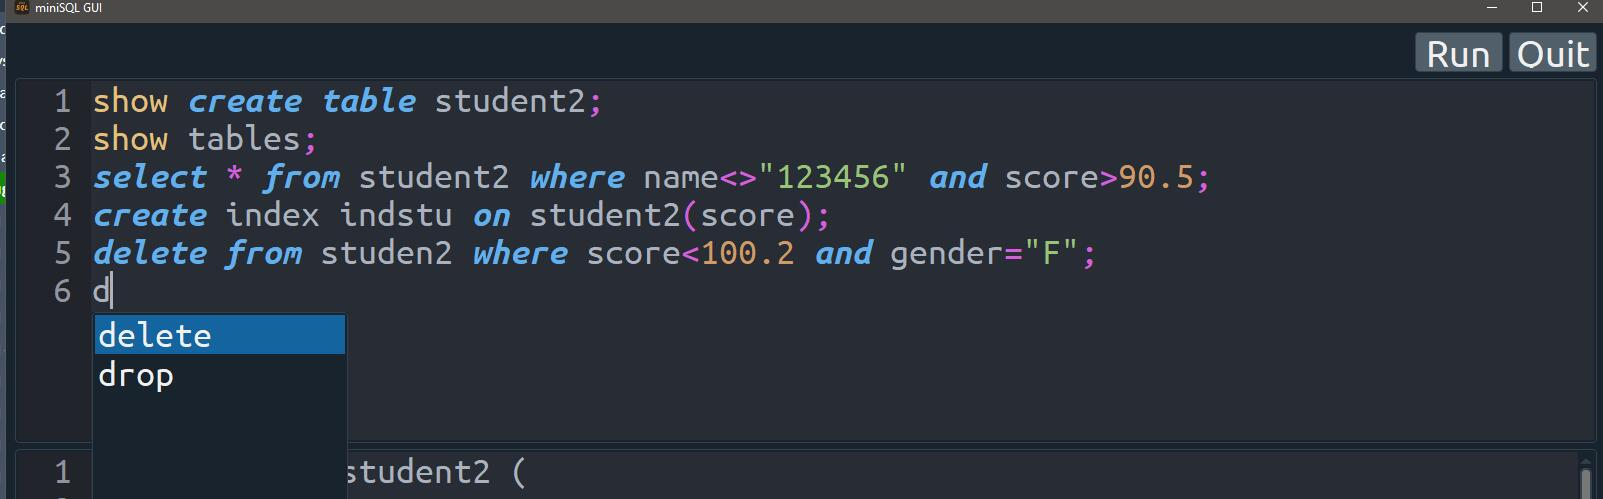
\includegraphics[width=\linewidth]{figure/editor_requirements.jpg}
    \caption{Editor Requirements}
    \label{fig:editor_requirements}
\end{figure}

\subsection{关于错误提示}
我们希望错误提示以一种用户容易接受的格式呈现到程序上,例如在所有严重错误前加上Error标识符。
结合GUI我们将会对这些格式化的错误信息进行高亮以方便用户识别。
\begin{figure}[H]
    \centering
    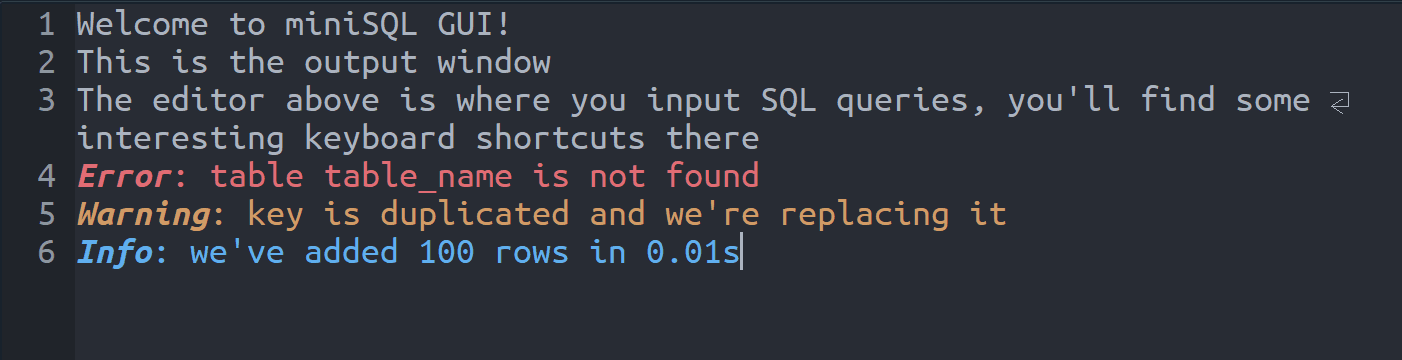
\includegraphics[width=\linewidth]{figure/error_requirements.png}
    \caption{Error Message Requirements}
    \label{fig:error_message_requirements}
\end{figure}

\chapter{实验环境}
\paragraph{主要开发语言}Python 3.7.*/3.8.*
\paragraph{主要开发环境}
\begin{itemize}
    \item PyCharm 2020.1
    \item Visual Studio Code 1.45
\end{itemize}
\paragraph{经过测试的系统环境}
\begin{itemize}
    \item \textsc{Microsoft Windows [Version 10.0.18363.836]}
    \item \textsc{Ubuntu WSL2}
    \item \textsc{MacOS Catalina}
\end{itemize}
\paragraph{\texttt{Python}包要求}QScintilla, QDarkStyle, PyQt5
\paragraph{实验系统环境} \textsc{Microsoft Windows [Version 10.0.18363.836]}
\paragraph{实验处理器环境} Intel(R) Core(TM) i7-9750H CPU @ 2.60GHz 12 Logical Processors
\paragraph{实验内存环境} SODIMM 15.8GB/16.0GB
\paragraph{实验硬盘环境} KBG30ZMS512G NVMe TOSHIBA 512GB

\chapter{系统设计}
\section{功能描述}
\subsection{建立/删除索引}
实际的数据库应用中,有在建立表时创建索引和表中有数据情况下创建索引的需求。区别在于,前者不需要其他模块为索引管理器提供数据,仅仅需要分配一个新索引所需的内存和磁盘空间;而后者要求发出建立索引请求的模块提供相应的数据块。默认情况下我们以记录的行号作为B+树中键值对上的“值”,因此我们要求相应数据块是按照它们将来被查找的顺序提供的。
\paragraph{建立索引}
正如图\ref{fig:index_example}所示的\footnote{图\ref{fig:index_example}来源于\textit{Database System Concepts 6th Edition Abraham Silberschatz等。}}。为了方便演示,让我们用其中的第一列作为建立索引的数据集。我们会按顺序将提供的数据插入索引数据结构,因此在这一个键值对中,键为第一列数据值,如\textit{10101},而值为行号,如\textit{0}。
\begin{figure}[H]
    \centering
    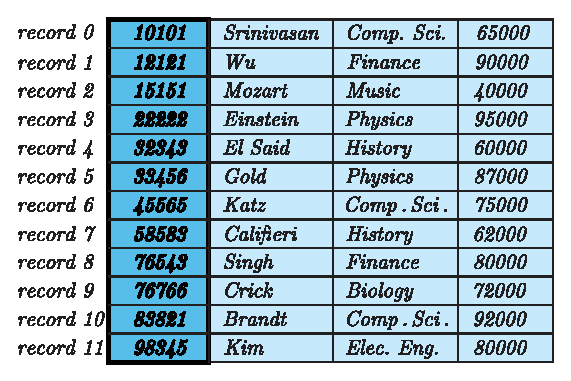
\includegraphics[width=0.7\linewidth]{figure/index_example.eps}
    \caption{线性记录储存方式}
    \label{fig:index_example}
\end{figure}

这样处理的原因在于,我们希望日后通过索引根据查找键快速找到记录对应的位置,而其在表格中的相对位置是最方便的寻址信息之一。若我们按照索引的自定义值储存插入的键,则索引失去加快搜索的作用;若我们插入的值为记录的绝对磁盘位置信息,则缓存管理器失效,且数据的移动会导致索引失效。
\par
在内存中创建索引(并插入相应数据后),索引管理器会将索引的内存信息叫给缓存管理器,由其决定是否应将内存保留或者存储到磁盘中,同时返回给索引管理器一个唯一的索引标号(索引管理器会将其继续返回给上层模块),日后将根据这一唯一标识符从缓存管理器中取得相应索引(无论是通过读取磁盘文件还是直接获取内存指针)。
\paragraph{删除索引}
我们通过上述的唯一标识符给缓存管理器发出删除信号,完成删除操作。

\subsection{查找/删除索引键}
查找和删除操作支持快速范围操作,并且两者在具体实现上有极大相似性,我们通过抽象两者的操作来提高代码复用率。
我们首先直接判断用户进行的是范围还是单值查找,并且替前从缓存管理器中取得相应索引内容(内存或硬盘中)。
\paragraph{单值操作}
我们调用B+树相应查找接口获得应查找的值,并通过异常来进行错误通讯。若查找成功则直接返回,否则抛出相关异常。
\begin{figure}[H]
    \centering
    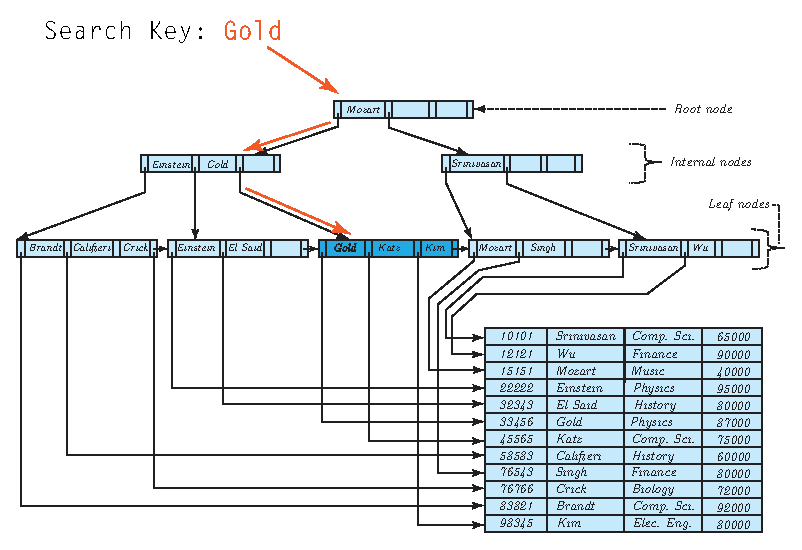
\includegraphics[width=0.75\linewidth]{figure/search_delete_single.eps}
    \caption{单值操作}
    \label{fig:search_delete_single}
\end{figure}


\paragraph{范围操作}
我们首先会检查用户给予的范围是否有效\footnote{例如,范围左右下标是否为左 小右大,或被查找的树是否为空等},同样的,我们使用异常来进行错误通讯,这使得接口模块能方便的实现错误处理。接着我们查询范围两端的值\footnote{我们默认范围查找的区间是左闭右开的。}并根据返回的节点情况进行相关操作,对于查找指令,这一操作是返回查询得到的相关信息;对于删除指令,这一操作是操作B+树删除相关的值,并在操作全部完成后将修改后的索引叫给缓存管理器。如图\ref{fig:search_delete_multi}所示(加深部分为需要查找或删除的部分)。

\begin{figure}[H]
    \centering
    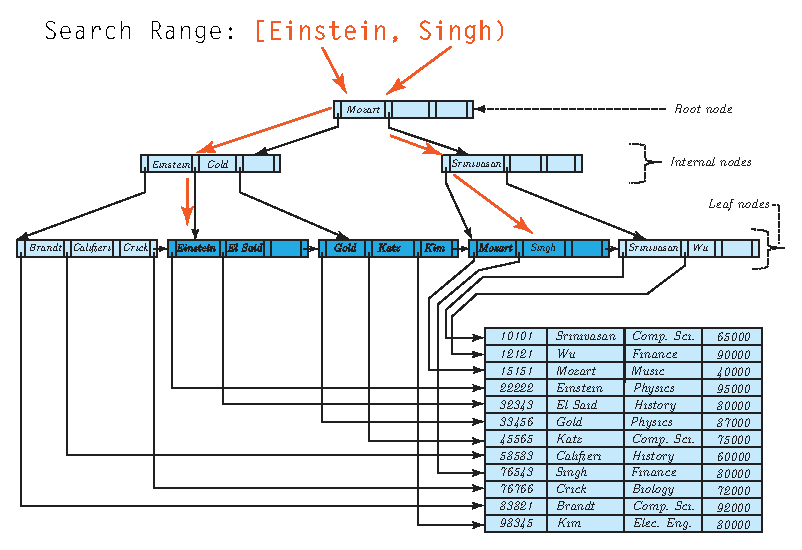
\includegraphics[width=0.75\linewidth]{figure/search_delete_multi.eps}
    \caption{范围操作}
    \label{fig:search_delete_multi}
\end{figure}

\subsection{插入键值对}
我们单独实现了插入键值对功能,因为其逻辑相对于查询和删除操作都有所不同(需检查重复元素等)。类似的,索引管理器会首先向缓存管理器请求相关索引内容。接着我们调用插入操作,将是否允许替换的信息传递给B+树的相关寒函数直接进行操作\footnote{原因在于B+树内部实现中也需要调用查找相关功能,与其规定执行流程,不如让B+树具体实现获得最优执行流程}。

\subsection{更新值内容}
由于我们使索引中键值对中\textit{值}指向记录在某张表中的位置,而这一位置在数据库运行过程中可能会发生很大变化\footnote{例如闲时的数据库清理和记录重排序等,亦或记录管理器采取了不同的数据储存模型。},我们给外界留出批量修改值的接口。
\par
这一操作类似于范围操作中涉及到的内容,我们需要对B+中的有效节点数目进行检查,根据节点数目选取不同的处理方式。

\subsection{图形界面}
我们拓展了API模块的接口,通过图形界面来提高用户体验。我们设计了一个编辑器界面,加入了语法提示与自动补全。我们通过\texttt{PyQt}来实现对图形界面的构建。

\subsection{缓存管理器}
我们估计一条记录占用空间大小为定值16字节,每块(block)大小固定为4K,则每一个块中有固定记录条数256条。同时,设置内存中最多能够存储的数据块数为2048块,因此内存中数据占用的空间最大为8M,处于可以接受的范围内。这样一来,当缓存管理器进行内部管理时,我们就可以用元组[表名, 块位置, 记录位置]来唯一标识任意一条记录的物理位置,如下图1所示(事实上,每个表的块数也限制为2048,即每个表最多可以有50万条记录,对于miniSQL,这是足够大的):
\begin{figure}[H]
    \centering
    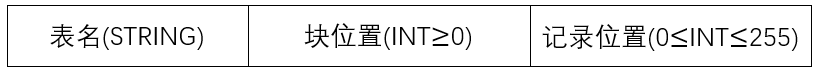
\includegraphics[width=0.75\linewidth]{figure/Position.jpg}
    \caption{记录位置的唯一标识}
    \label{fig:Position}
\end{figure}
为了方便模块间的信息传递,每一条记录也可以用元组[表名, 位置]来唯一标识,此时我们有:

\textbf{位置 $=$ 块位置 ${\times256}$ + 记录位置}

从而,无论是缓存和记录管理器之间,还是和索引管理器的信息交互,对于任一表中的任一条记录,我们总是用一个整数‘位置’来唯一标识它,且可以和图1中的表示任意转化。

\paragraph{记录取得(Get Blocks)}
当某一表的记录被查询/删除/搜索时,缓存管理器收到记录管理器的信息,并返回所需要的块列表。由于记录在文件中的排列顺序相对随机,我们设计选择返回所需表的全部记录块给记录管理器。这可以通过遍历内存中的所有数据块和相应文件中的数据块(如有必要)实现。

当内存中不包含该表的全部记录信息(即块信息)时,必须要访问相应的表文件取得数据块。更进一步地,当内存中可以存储的块数满时,我们必须要换进换出数据块。需要注意的是,我们总是保证文件中的记录位置最大值大于等于缓存中的,这为脏数据块的写回(write back)提供的便利。

\paragraph{记录插入(Insert Records)}
当一条记录被插入时,缓存管理器收到记录管理器的信息。若该表中间的每一条记录都是有效(包括无记录被删除过或被删除记录的位置已全部被新纪录填充两种情况)插入记录至表的最后一行并总是将记录插入到文件末尾(记录插入文件通过调用文件管理器中相应接口完成),否则插入记录至之前被删除记录的无效位置。

在记录被删除时,为防止其他记录的位置变动,我们选择懒惰删除的形式。这就需要一个数据结构存储被删除的记录位置。因此,在插入记录时,我们必须要考虑之前是否曾经删除过记录。同时,为了搜索的方便(这是由记录取得(Get Blocks)的实现方式决定的),当在表的最后插入记录时,总是要求也将记录插入文件的末尾,以保证缓存的记录位置最大值不会超过文件中的。

插入完成后,缓存管理器返回新记录的‘位置’信息。

\paragraph{最近最少用(Least Recently Used)}
当内存中数据块个数达到预设的最大值时,需要选择合适的块进行替换。我们总是假设最近访问的块是最有可能再次访问的,因而选择使用最近最少用策略进行块替换。

具体而言,即选择访问时间最早的块进行替换操作,且当所选择的块为脏(dirty)块时(即该块中的内容比文件中新),需要先写回文件再进行替换。

\paragraph{保存/取得/删除索引(Save/Get/Delete Indexes)}
对于索引,更准确的说,是某个表上某属性的B+树结构,为了尽量减少与文件系统的交互,提高效率,我们选择将全部索引信息存储在内存中,不作数量限制,这在表数不多时是可以接受的。只在miniSQL系统启动时从文件读入全部信息,在系统关闭(或空闲)时存储全部信息至文件。

因此,保存/取得/删除索引的操作均只需要对内存进行操作即可,用Python自带的字典数据结构可以非常容易地根据索引编号找到对应的B+树,进行所需的操作。

\subsection{记录管理器}
\paragraph{删除/查询记录}	
对从缓存管理器取得的数据块列表进行按条件分析筛选,取出符合条件的记录。筛选过程基本一致,区别在于最后删除记录返回的是被删除记录的‘位置’号列表(并加入freeList中),查询记录返回的是记录本身构成的列表。

\paragraph{插入记录}
调用缓存管理器完成记录的插入,不需要返回任何信息。

\paragraph{创建/删除/清空表}
调用缓存管理器中DataBuffer对象的成员函数完成,不需要返回任何信息。

\section{主要数据结构}
\subsection{B+树}
\footnote{此段内容摘自\href{https://en.wikipedia.org/wiki/B+_tree}{WikiPedia}}
B+ 树是一种树数据结构,通常用于数据库和操作系统的文件系统中。B+ 树的特点是能够保持数据稳定有序,其插入与修改拥有较稳定的对数时间复杂度。B+ 树元素自底向上插入,这与二叉树恰好相反。
\par
B+ 树在节点访问时间远远超过节点内部访问时间的时候,比可作为替代的实现有着实在的优势。这通常在多数节点在次级存储比如硬盘中的时候出现。通过最大化在每个内部节点内的子节点的数目减少树的高度,平衡操作不经常发生,而且效率增加了。这种价值得以确立通常需要每个节点在次级存储中占据完整的磁盘块或近似的大小。
\par
B+ 背后的想法是内部节点可以有在预定范围内的可变量目的子节点。因此,B+ 树不需要像其他自平衡二叉查找树那样经常的重新平衡。对于特定的实现在子节点数目上的低和高边界是固定的。例如,在 2-3 B 树(常简称为2-3 树)中,每个内部节点只可能有 2 或 3 个子节点。如果节点有无效数目的子节点则被当作处于违规状态。
\par
B+ 树的创造者 Rudolf Bayer 没有解释B代表什么。最常见的观点是B代表平衡(balanced),因为所有的叶子节点在树中都在相同的级别上。B也可能代表Bayer,或者是波音(Boeing),因为他曾经工作于波音科学研究实验室。

\paragraph{查找}
查找以典型的方式进行,类似于二叉查找树。起始于根节点,自顶向下遍历树,选择其分离值在要查找值的任意一边的子指针。在节点内部典型的使用是二分查找来确定这个位置。

\paragraph{插入}
节点要处于违规状态,它必须包含在可接受范围之外数目的元素。
首先,查找要插入其中的节点的位置。接着把值插入这个节点中。
如果没有节点处于违规状态则处理结束。
如果某个节点有过多元素,则把它分裂为两个节点,每个都有最小数目的元素。在树上递归向上继续这个处理直到到达根节点,如果根节点被分裂,则创建一个新根节点。为了使它工作,元素的最小和最大数目典型的必须选择为使最小数不小于最大数的一半。

\paragraph{删除}
首先,查找要删除的值。接着从包含它的节点中删除这个值。
如果没有节点处于违规状态则处理结束。
如果节点处于违规状态则有两种可能情况:
它的兄弟节点,就是同一个父节点的子节点,可以把一个或多个它的子节点转移到当前节点,而把它返回为合法状态。如果是这样,在更改父节点和两个兄弟节点的分离值之后处理结束。
亦或,它的兄弟节点由于处在低边界上而没有额外的子节点。在这种情况下把两个兄弟节点合并到一个单一的节点中,而且我们递归到父节点上,因为它被删除了一个子节点。持续这个处理直到当前节点是合法状态或者到达根节点,在其上根节点的子节点被合并而且合并后的节点成为新的根节点。

\subsection{排序数组}
本数据结构是为了配合主键而实现的,采用最普通的排序数组查找方式,并在数组内部采用二分查找进行相关操作。
可从无限子树数目的B+树抽象的到,因此我们可以较为方便的统一两者的接口。
\par
值得注意的是,为了配合主键和记录管理器中数据的储存方式,我们往往使用一种特殊的类作为排序数组的内部容器:一种返回当前下标的特殊数组\footnote{我们可以利用这一特性而使得这种储存不占用任何空间,而同时保证接口的一致性。}。

\subsection{数据块类(Class DataBlock)}
本数据结构是缓存管理器保存数据的重要组成部分,其数据成员如下:
\begin{itemize}
	\item 锁位(pin):表示该块是否被锁住,即不能被替换。为布尔(bool)类型。
	\item 脏位(dirty):表示该快的内容是否比文件中更加新,即是否被操作改变过但还未写回文件。为布尔(bool)类型。
	\item 表名(tablename):该块所对应的表名。为字符串(String)类型。
	\item 位置(position):块位置。为整数(int)类型。
	\item 内容(content):块的内容,包含该块的全部(最新)记录信息。为列表(list)类型,其中的每个元素均为一条记录元组,在列表中的位置对应在磁盘中的物理位置。
	\item 最近访问时间(Last Access Time, LAT):记录该块最近一次被访问的时间。
\end{itemize}

\subsection{数据缓存类(class DataBuffer)}
本数据结构是缓存管理器数据管理的重要部分,以数据块类为主体,通过对数据块与文件之间的交互管理,提高了执行效率,其数据成员和成员函数如下:
\begin{itemize}
	\item 数据缓存(buffer):一个存储数据块类的列表(list),列表元素数最大为2048。
	\item 数据块数(blockNum):当前缓存中已有的数据块数,即数据缓存列表的元素数,为了方便作为数据成员单独列出。
	\item 整个缓存查找替换(LRU):遍历数据缓存,找到访问时间最早的块,若是脏的,写回;最后将该块在列表中删除。
	\item 记录插入(insert\_record):插入记录。
	\item 整个缓存除某表外替换(LRU\_except\_one):遍历除某一表外的数据缓存块,进行LRU操作。
	\item 记录取得(get\_blocks):取得某表的全部数据块。
	\item 创建表(create\_table):创建一个新的表(调用文件管理器)。
	\item 删除表(delete\_table):删除一个现有表(调用文件管理器)。
	\item 清空表(clear\_table):清空一个现有表的全部数据(调用文件管理器)。
\end{itemize}

\subsection{缓存管理器中的其它数据结构}
\paragraph{freeList} 为一个字典,键值对为[表名:对应已删除元素的列表]。
\paragraph{index\_buffer} 为一个字典,键值对为[标号:对应B+树]。
\paragraph{maxrecordNum} 为一个字典,键值对为[表名:该表记录最大‘位置’号]。

\subsection{条件类(Class Condition)}
本数据结构对记录管理器筛选数据起着重要作用,其数据成员如下:
\begin{itemize}
	\item 属性(attribute):记录是该表第几个属性上的条件,为一个整数。
	\item 类型(type):记录条件的类型(等于,小于,大于等),为一个整数。
	\item 值(value):条件中参与比较的值。
\end{itemize}

\section{类图与类间关系}
\subsection{B+树}
B+树的类图实现如图\ref{fig:bplus_diagram}所示\footnote{为了类图完整性,我们也列举了除用户自定义类型以外的类型。}\footnote{我们使用矢量图渲染了字体,若图表过小请放大查看。}。
\begin{figure}[H]
    \centering
    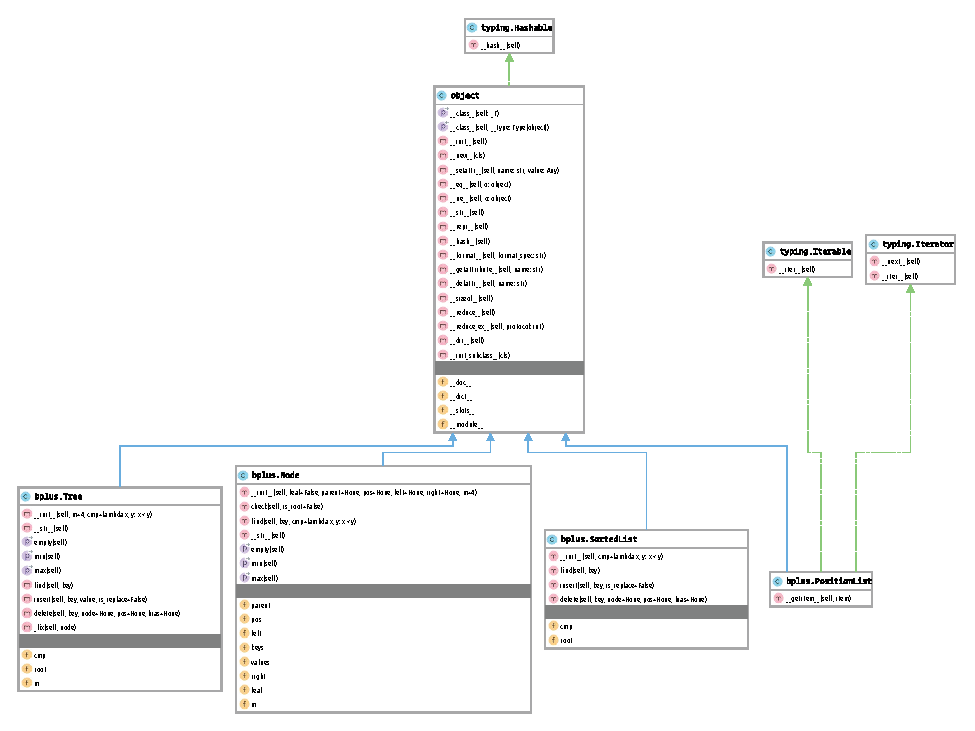
\includegraphics[width=\linewidth]{figure/bplus.eps}
    \caption{B+树的类图与类间关系}
    \label{fig:bplus_diagram}
\end{figure}
\subsection{异常类型}
程序使用的异常类图如\ref{fig:exceptions_diagram}所示。
\begin{figure}[H]
    \centering
    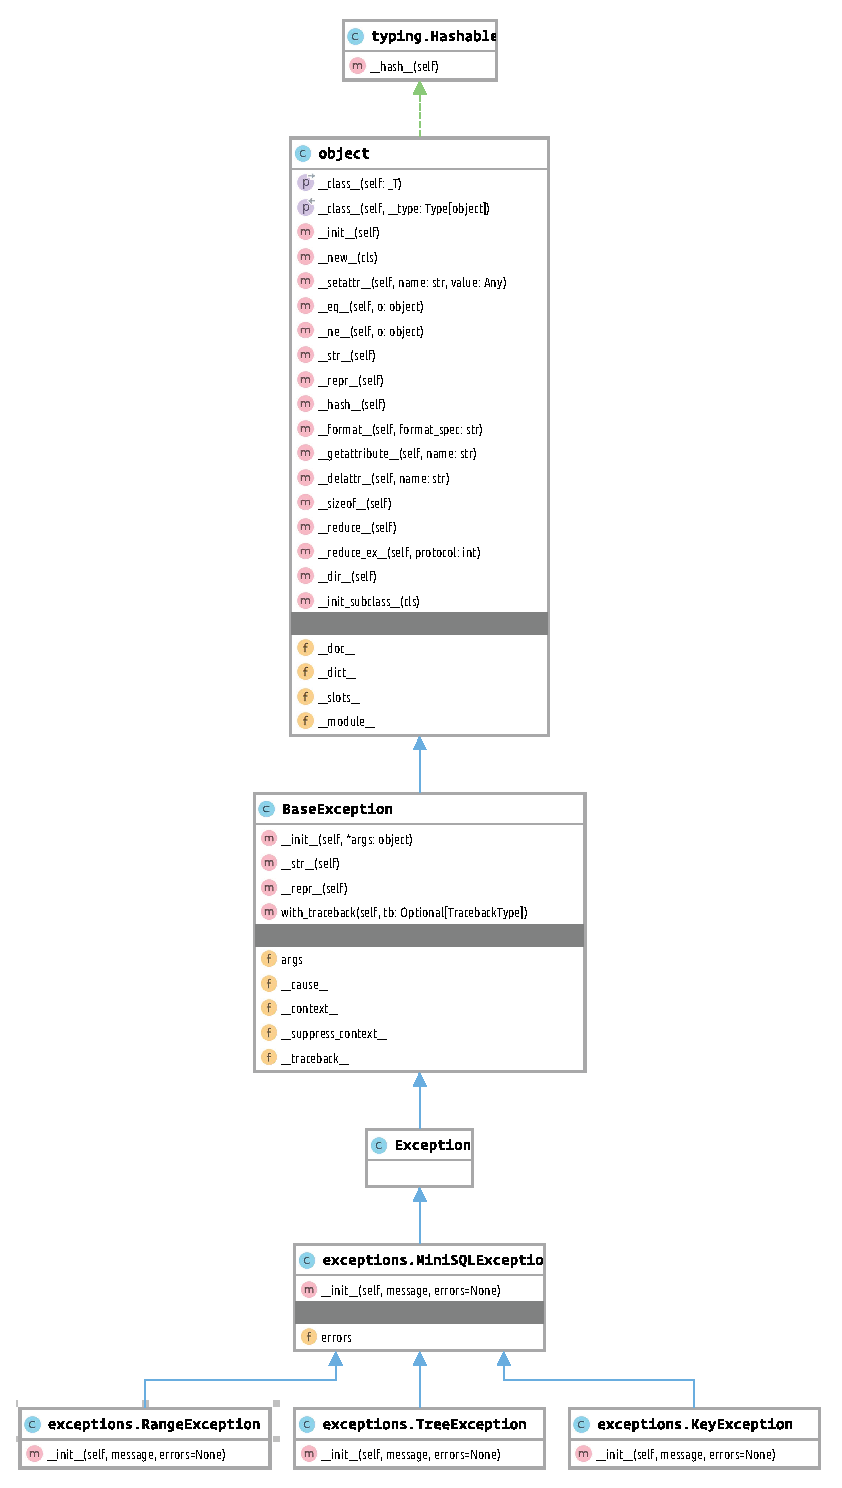
\includegraphics[width=0.7\linewidth]{figure/exceptions.eps}
    \caption{异常的类图与类间关系}
    \label{fig:exceptions_diagram}
\end{figure}
\subsection{索引管理器}
在具体的索引管理器实现上,我们采用了模块层面上的抽象而非类层面的,这更贴合\texttt{Python}语言的风格。
这样能保证尽量大的抽象层次与代码复用率。值得注意的是,我们在实现B+树相关操作的时候也使用了静态函数来抽象部分内容\footnote{我们将在下一部分详细阐述实现细节}。

\subsection{图形界面}
\begin{figure}[H]
    \centering
    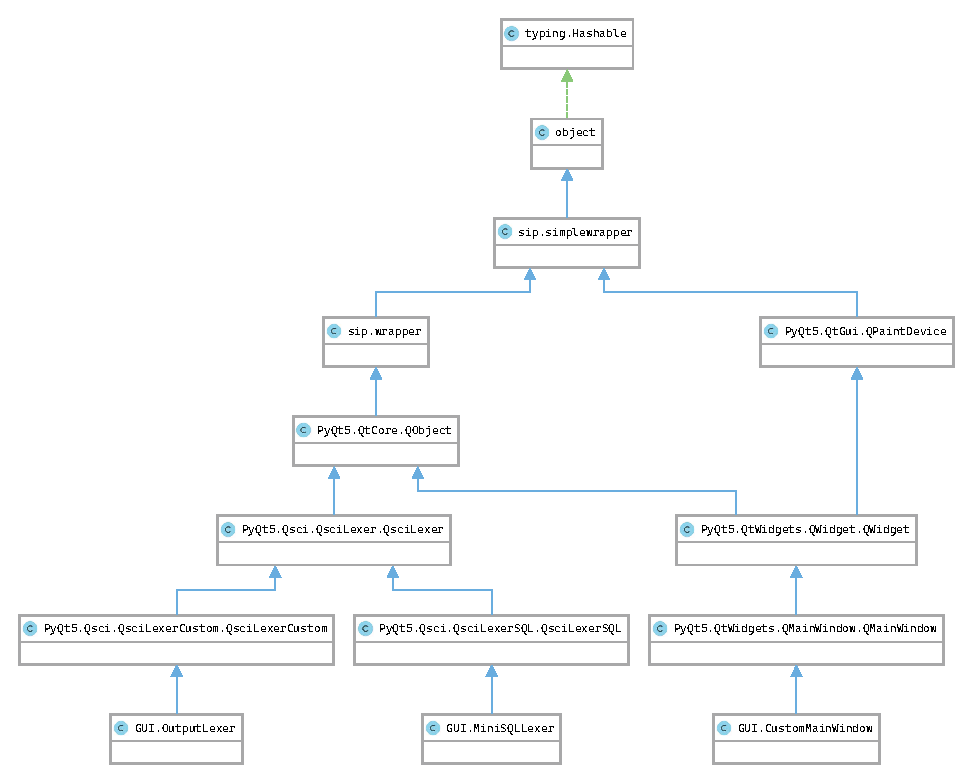
\includegraphics[width=\linewidth]{figure/gui_class.eps}
    \caption{图形界面类图}
    \label{fig:gui_class}
\end{figure}

\subsection{缓存管理器}
在具体的缓存管理器实现上,我们采用了类层面上的抽象,尽可能多的利用类成员函数解决问题。
\begin{figure}[H]
    \centering
    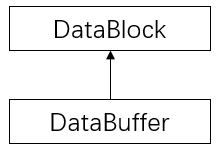
\includegraphics[width=0.25\linewidth]{figure/class1.jpg}
    \caption{缓存管理器类间关系}
    \label{fig:class1}
\end{figure}

\chapter{系统实现分析及运行截图}
\section{创建表语句}
\subsection{执行流程}
1.GUI读入,调用API;
\par
2.API调用interpreter解析并处理错误;
\par
3.返回API,调用catalog manager,record manager和index manager;
\par
4.record manager调用buffer manager,再由buffer manager调用file manager建表;
\par
5.index manager调用buffer manager建主键index;
\par
6.API计算运行时间,返回给GUI输出。
\subsection{运行截图}
\begin{figure}[H]
    \centering
    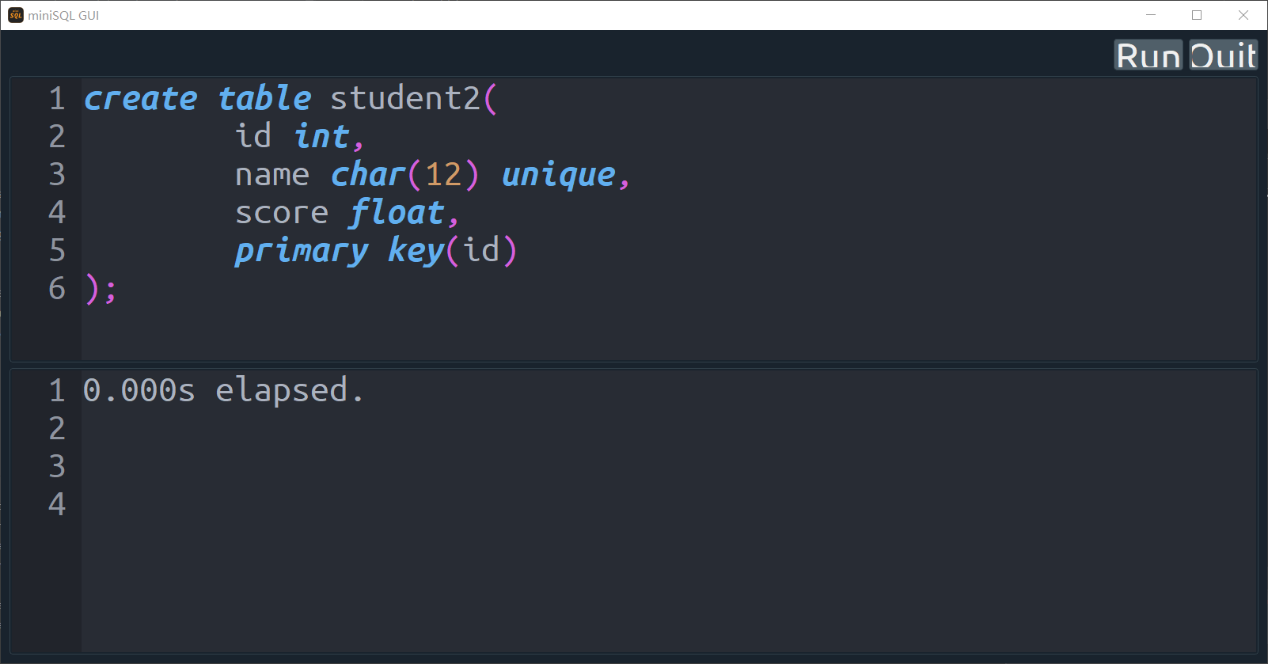
\includegraphics[width=0.8\linewidth]{figure/1.1.png}
    \caption{create table}
    \label{fig:runtime1.1}
\end{figure}
\section{删除表语句}
\subsection{执行流程}
1.GUI读入,调用API;
\par
2.API调用interpreter解析并处理错误;
\par
3.返回API,调用catalog manager得到要删除的表的index,调用index manager删除这些index(index manager将调用buffer manager);
\par
4.调用catalog manager 和record manager删除表(record manager将调用buffer manager并由buffer manager调用file manager进行删除);
\par
5.API统计执行时间,返回给GUI输出。
\subsection{运行截图}
\begin{figure}[H]
    \centering
    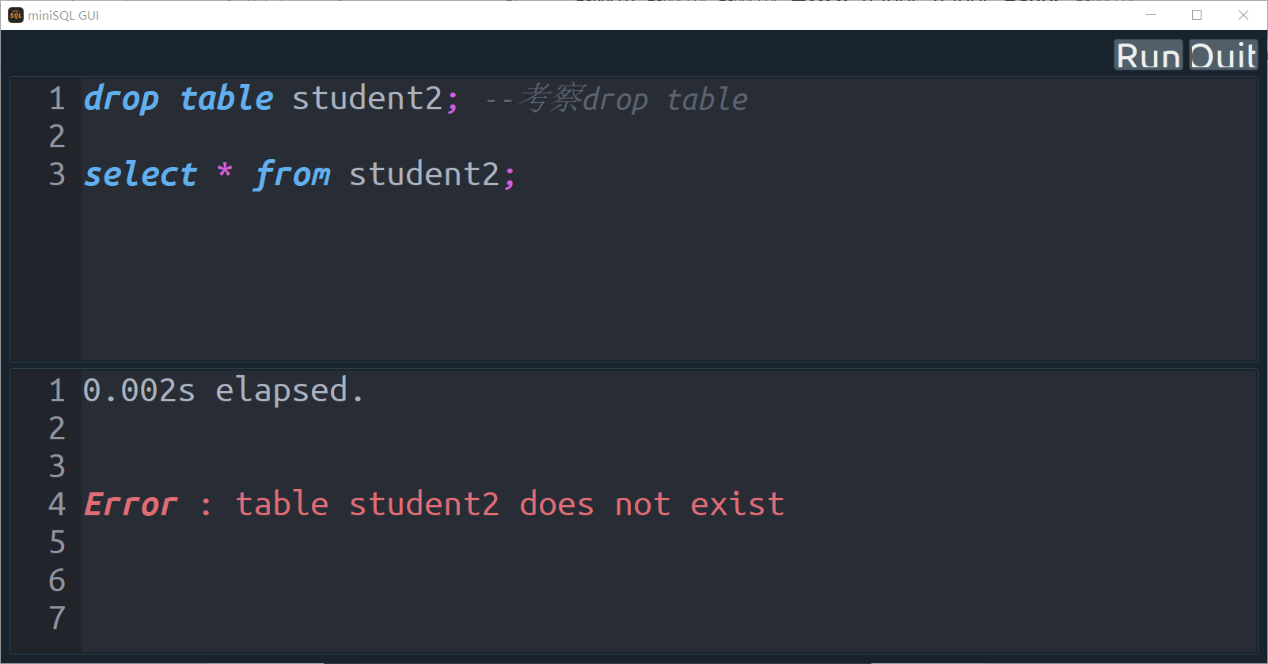
\includegraphics[width=0.8\linewidth]{figure/2.1.png}
    \caption{drop table}
    \label{fig:runtime2.1}
\end{figure}
\section{创建索引语句}
\subsection{执行流程}
1.GUI读入,调用API;
\par
2.API调用interpreter解析并处理错误;
\par
3.返回API,调用catalog manager建立index并返回index id,调用record manager得到要建index的attribute的数据,调用index manager对这些数据建立index;
\par
4.API统计执行时间,返回给GUI输出。
\subsection{运行截图}
\begin{figure}[H]
    \centering
    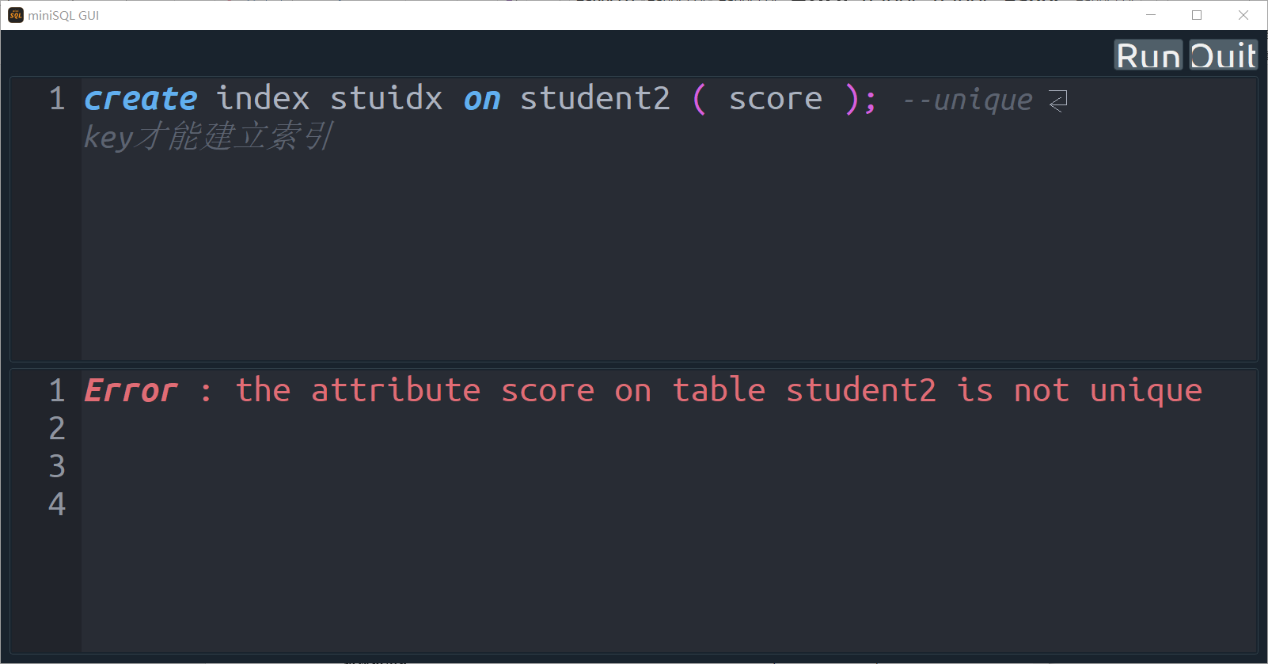
\includegraphics[width=0.8\linewidth]{figure/3.1.png}
    \caption{create index-failed}
    \label{fig:runtime3.1}
\end{figure}
\begin{figure}[H]
    \centering
    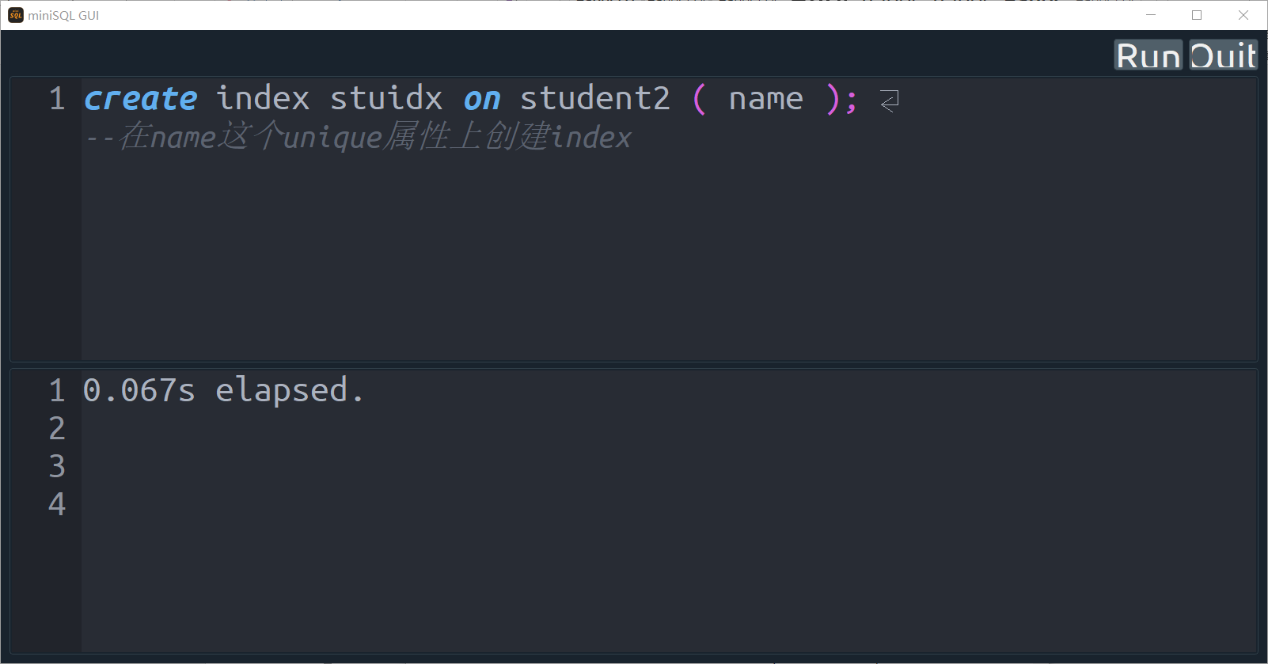
\includegraphics[width=0.8\linewidth]{figure/3.2.png}
    \caption{create index-succeed}
    \label{fig:runtime3.2}
\end{figure}
\section{删除索引语句}
\subsection{执行流程}
1.GUI读入,调用API;
\par
2.API调用interpreter解析并处理错误;
\par
3.返回API,调用catalog manager得到要删除的index的id并删除index,调用index manager根据id删除index(index manager将调用buffer manager);
\par
4.API统计执行时间,返回给GUI输出。
\subsection{运行截图}
\begin{figure}[H]
    \centering
    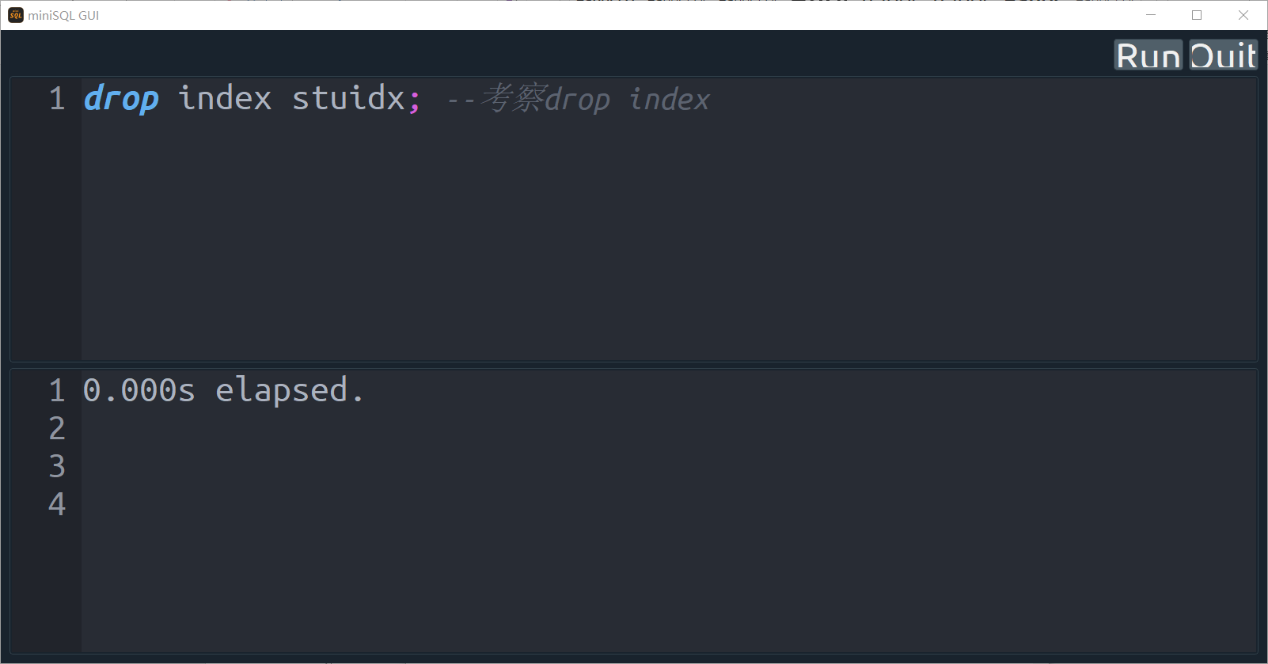
\includegraphics[width=0.8\linewidth]{figure/4.1.png}
    \caption{drop index}
    \label{fig:runtime4.1}
\end{figure}
\section{选择语句}
\subsection{执行流程}
1.GUI读入,调用API;
\par
2.API调用interpreter解析并处理错误;
\par
3.返回API,这里分为两种类型,一种是查询的attribute包含index的,一种是不包含index的;
\par
4.对于包含index的查询,调用index manager进行查询并返回查询结果的行号(将调用buffer manager),将行号和(可能有的)剩余的查询要求交给record manager进行查询(可能需调用buffer manager,并由buffer manager调用file manager得到数据block);
\par
5.对于不包含index的查询,直接调用record manager同上;
\par
6.API统计执行时间,返回给GUI输出。
\subsection{运行截图}
\begin{figure}[H]
    \centering
    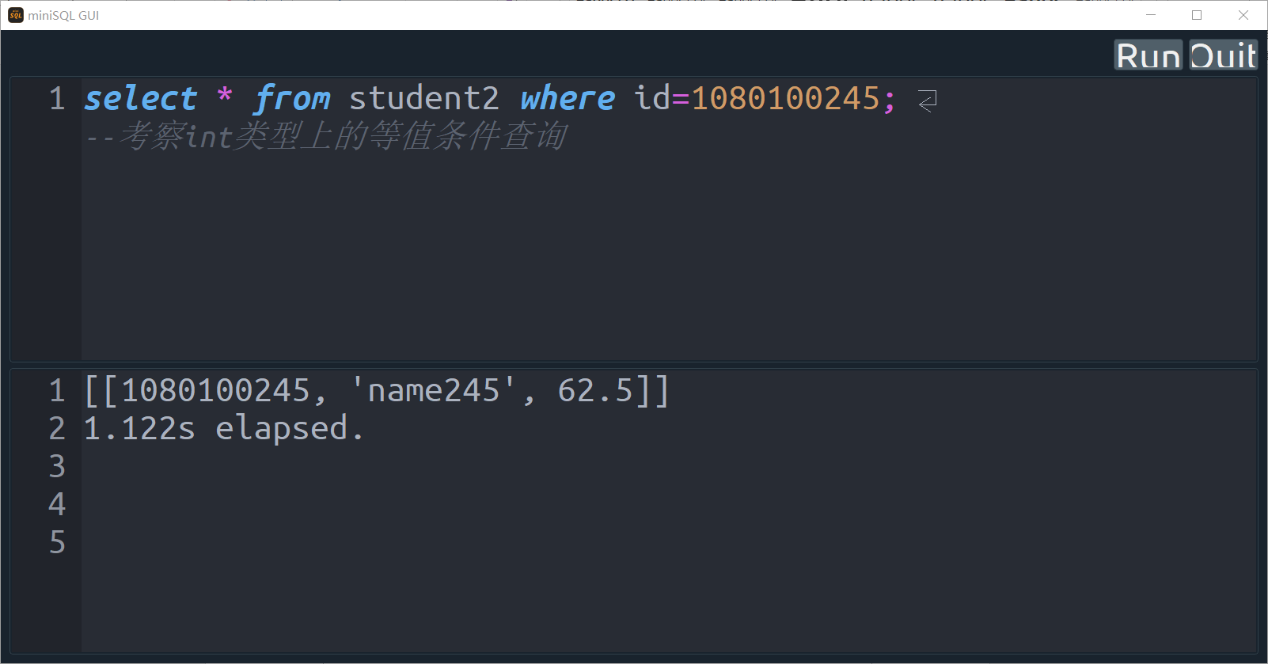
\includegraphics[width=0.8\linewidth]{figure/5.1.png}
    \caption{select-int+'='}
    \label{fig:runtime5.1}
\end{figure}
\begin{figure}[H]
    \centering
    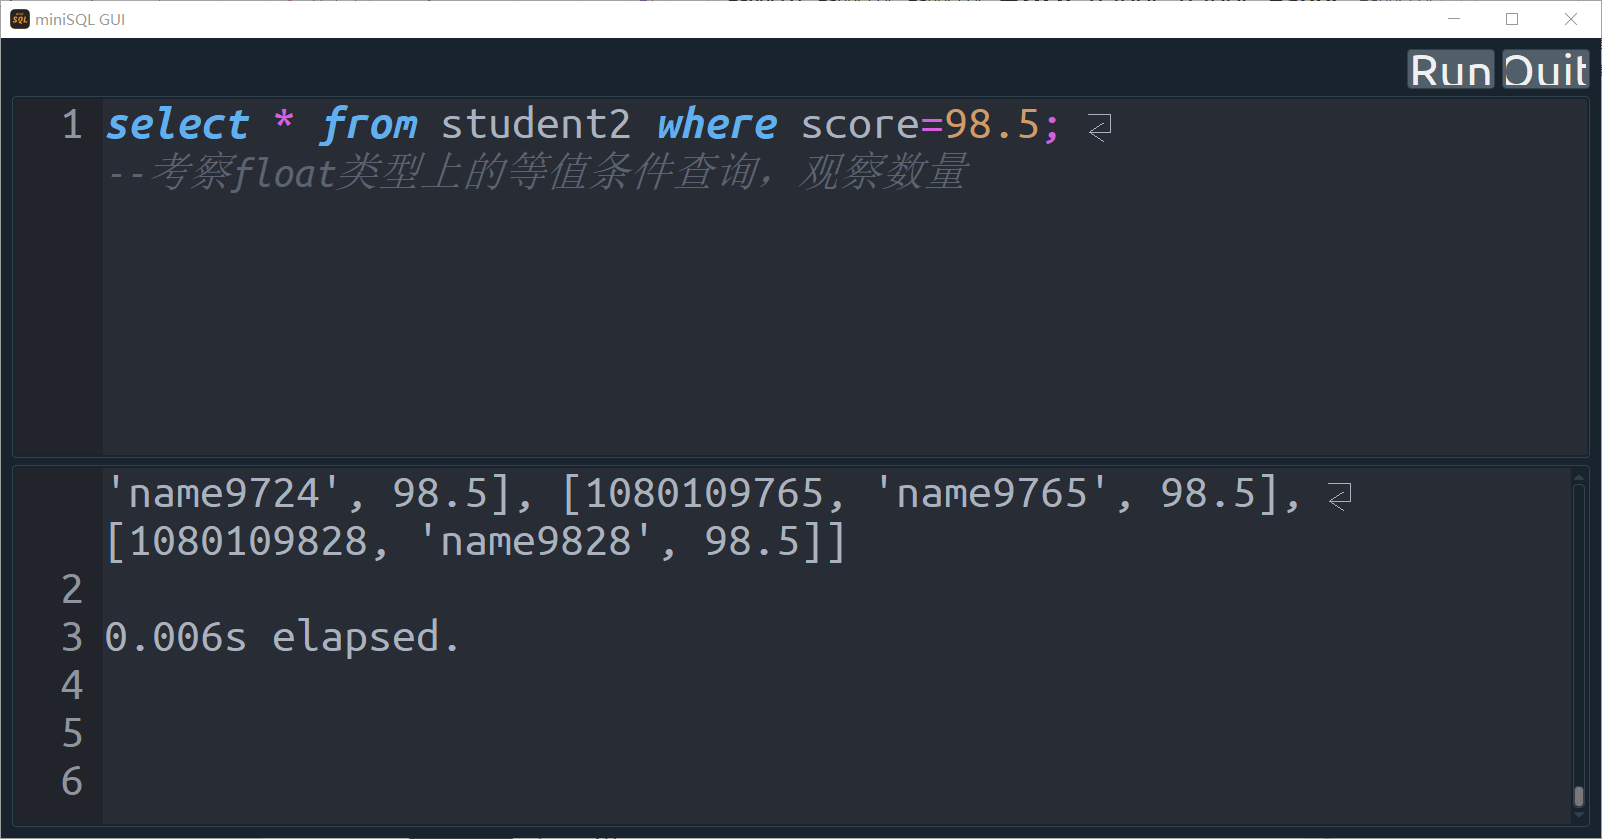
\includegraphics[width=0.8\linewidth]{figure/5.2.png}
    \caption{select-float+'='}
    \label{fig:runtime5.2}
\end{figure}
\begin{figure}[H]
    \centering
    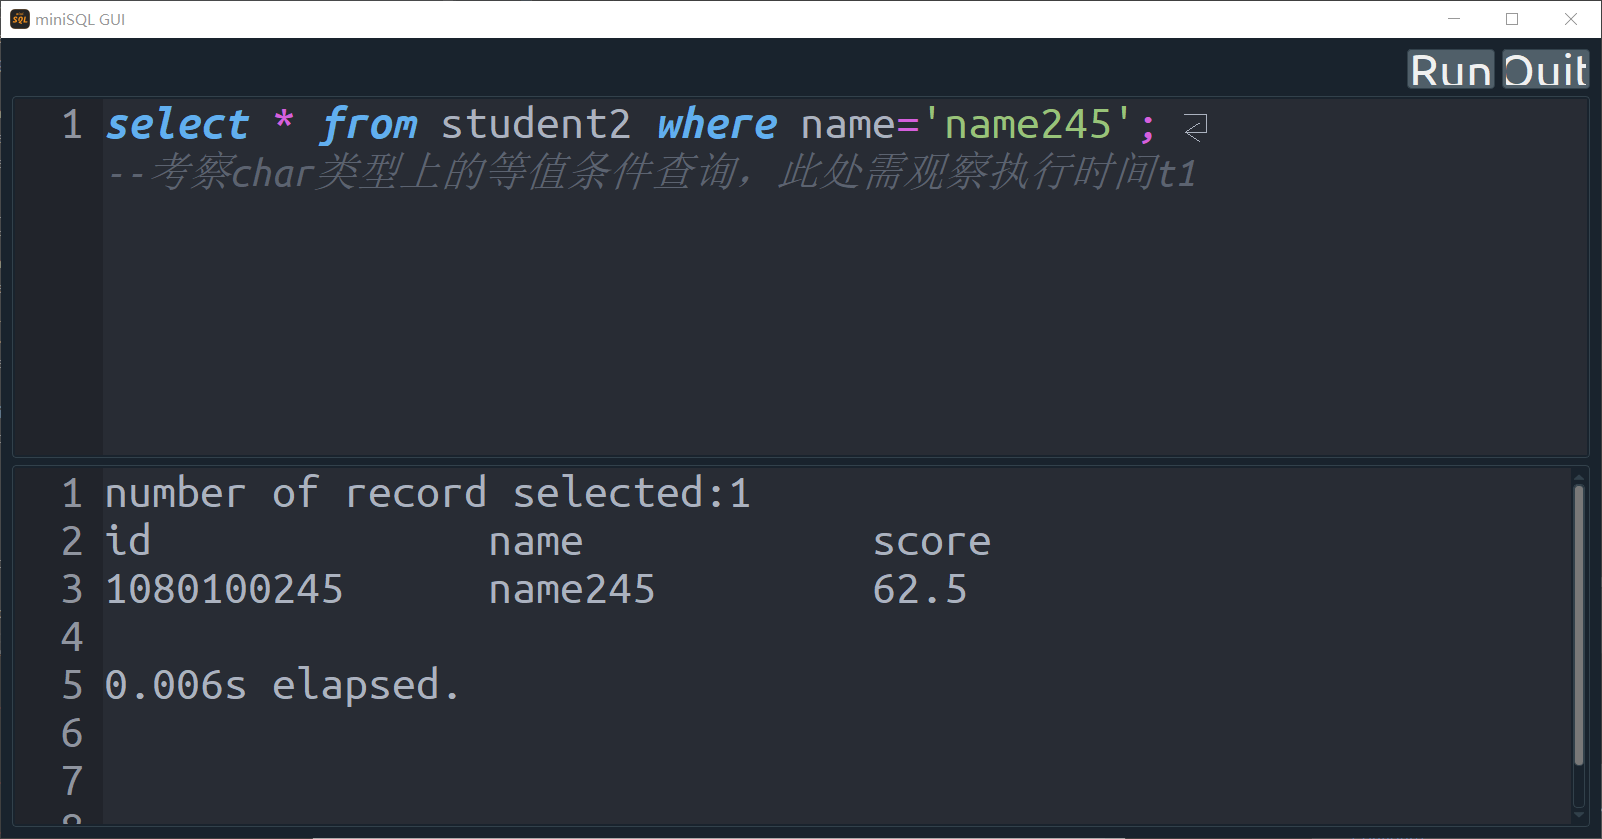
\includegraphics[width=0.8\linewidth]{figure/5.3.png}
    \caption{select-char+'='}
    \label{fig:runtime5.3}
\end{figure}
\begin{figure}[H]
    \centering
    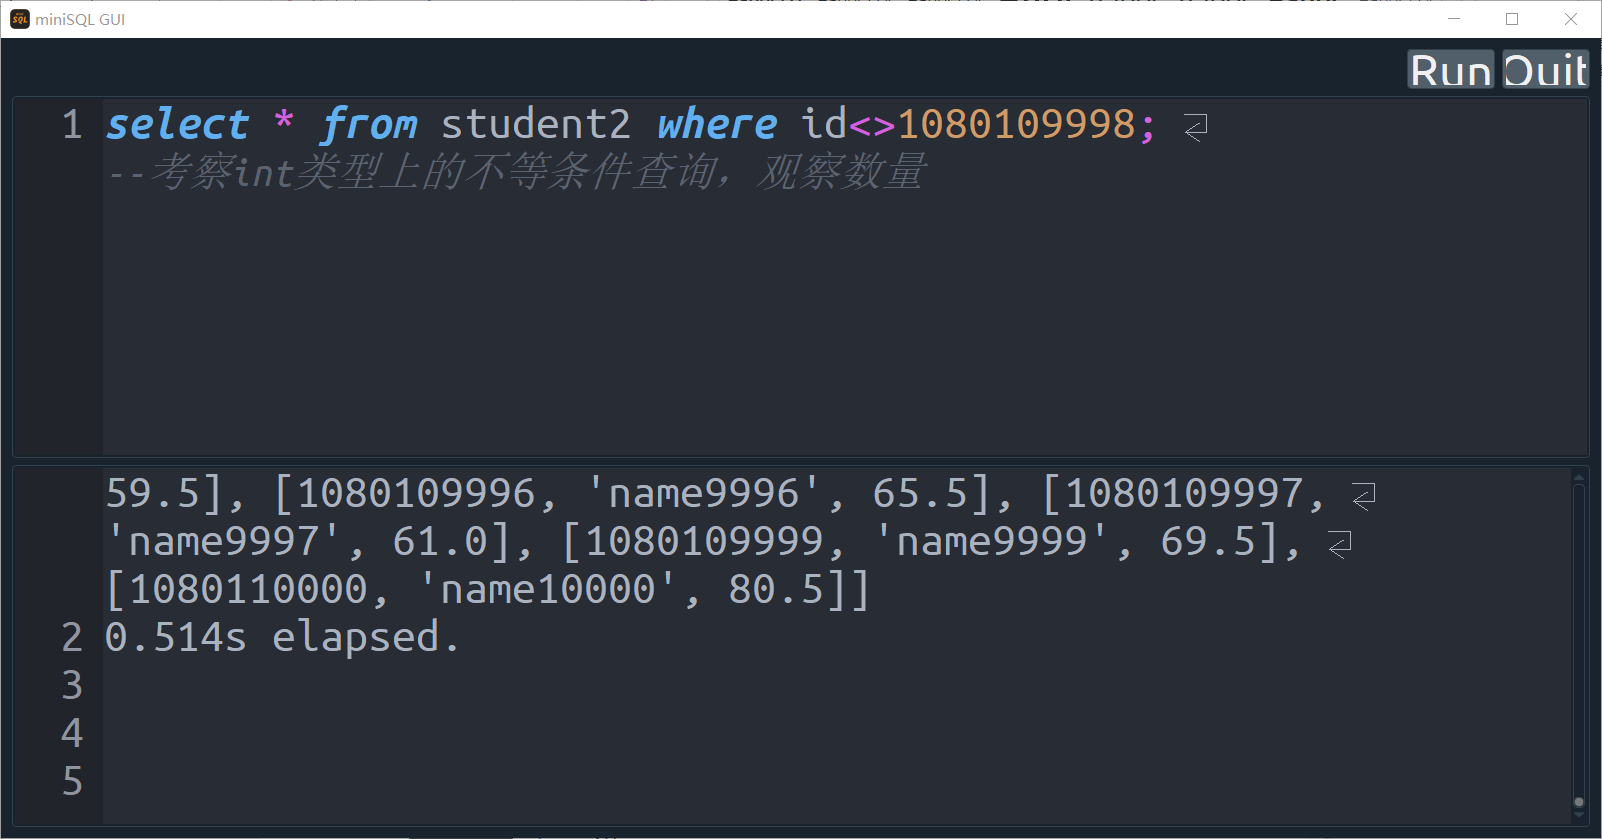
\includegraphics[width=0.8\linewidth]{figure/5.4.png}
    \caption{select-int+'<>'}
    \label{fig:runtime5.4}
\end{figure}
\begin{figure}[H]
    \centering
    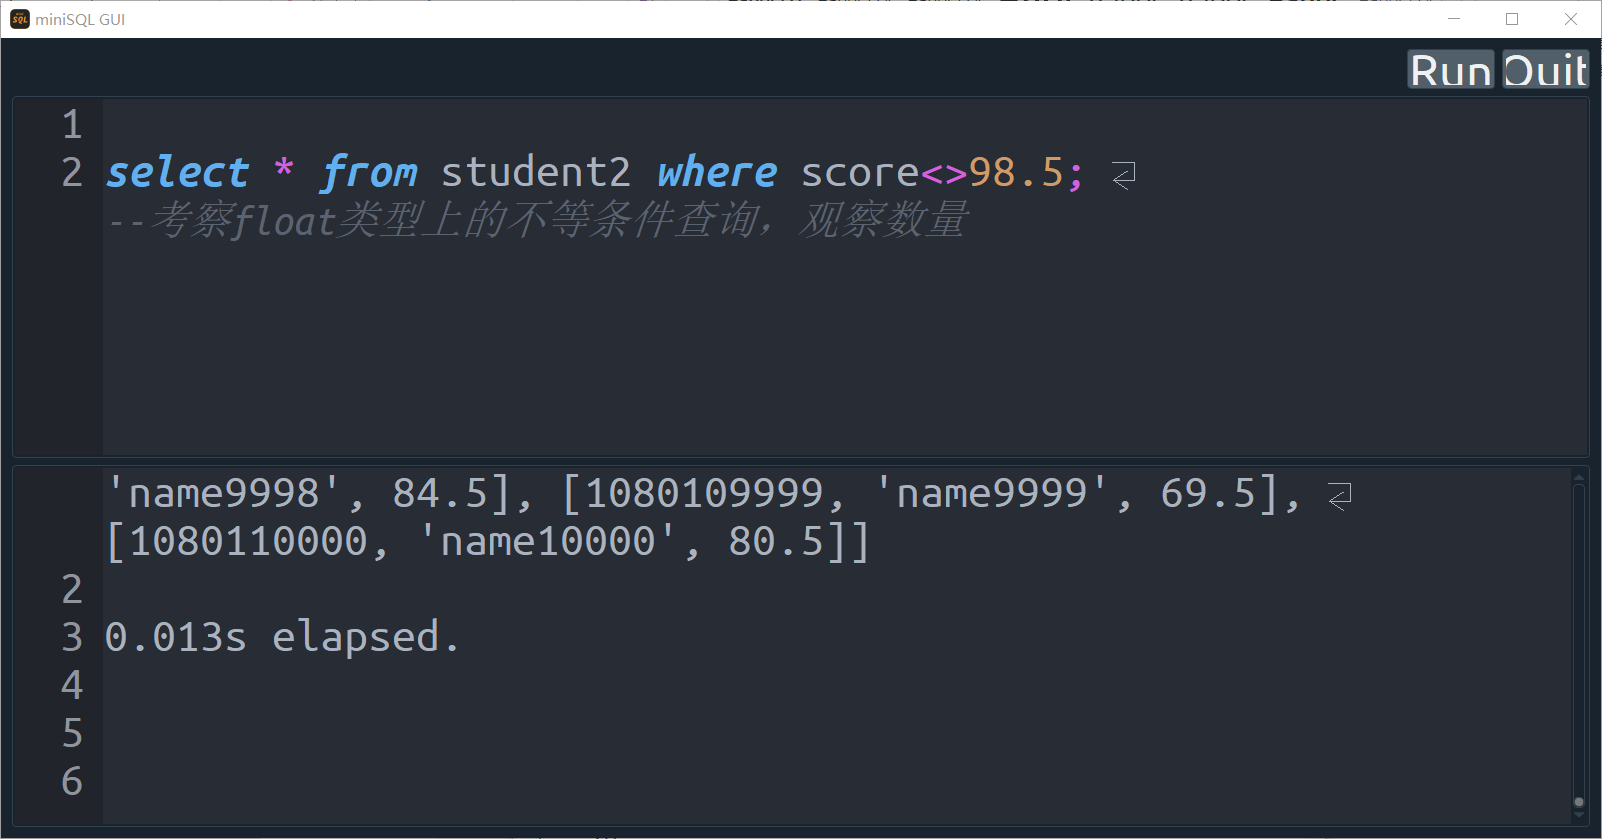
\includegraphics[width=0.8\linewidth]{figure/5.5.png}
    \caption{select-float+''<>}
    \label{fig:runtime5.5}
\end{figure}
\begin{figure}[H]
    \centering
    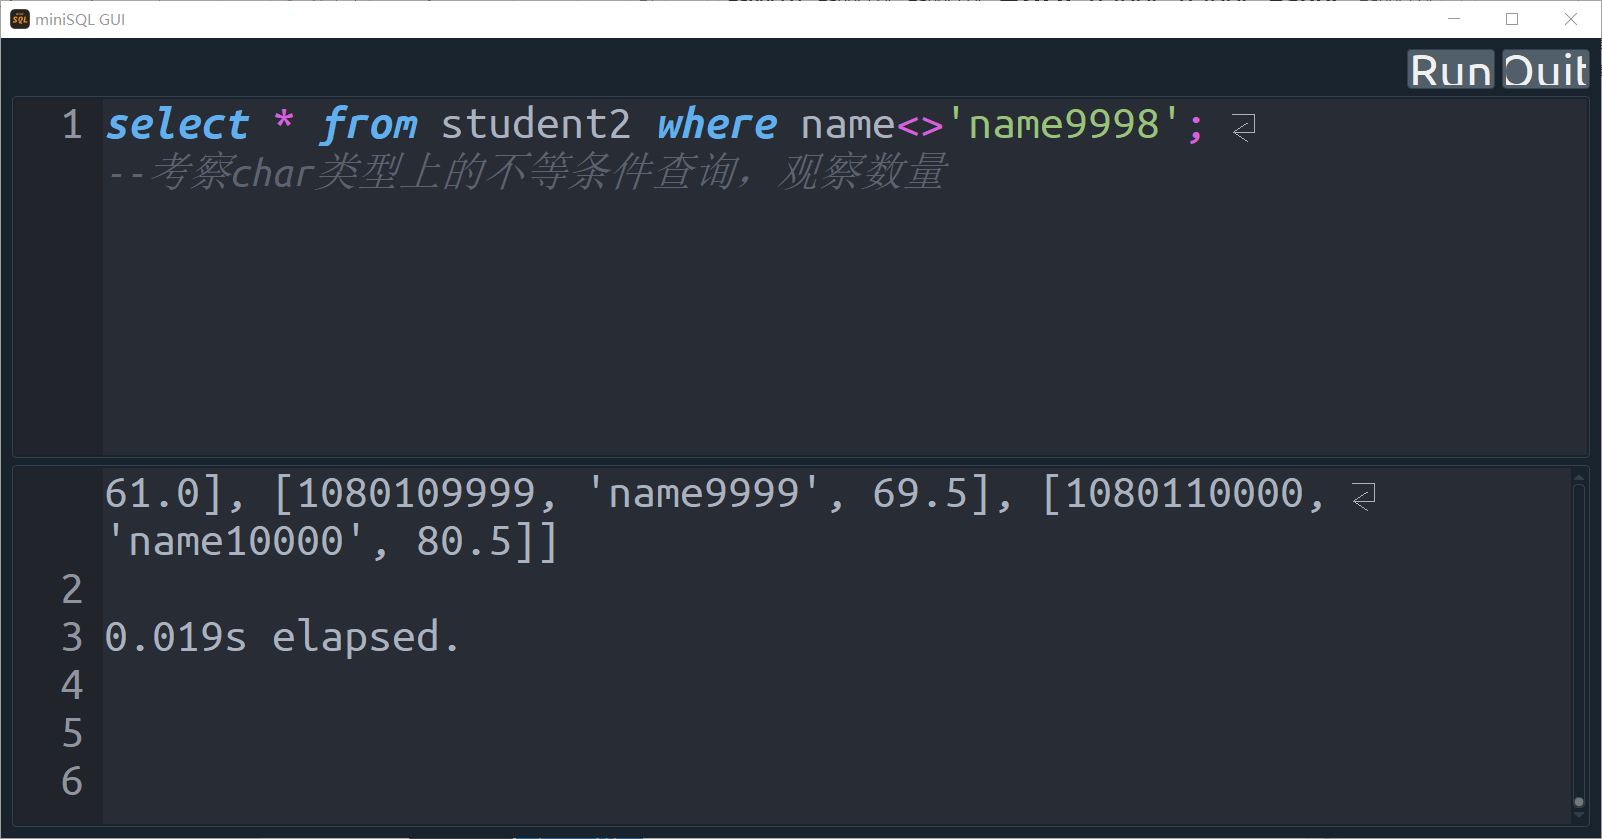
\includegraphics[width=0.8\linewidth]{figure/5.6.png}
    \caption{select-char+'<>'}
    \label{fig:runtime5.6}
\end{figure}
\begin{figure}[H]
    \centering
    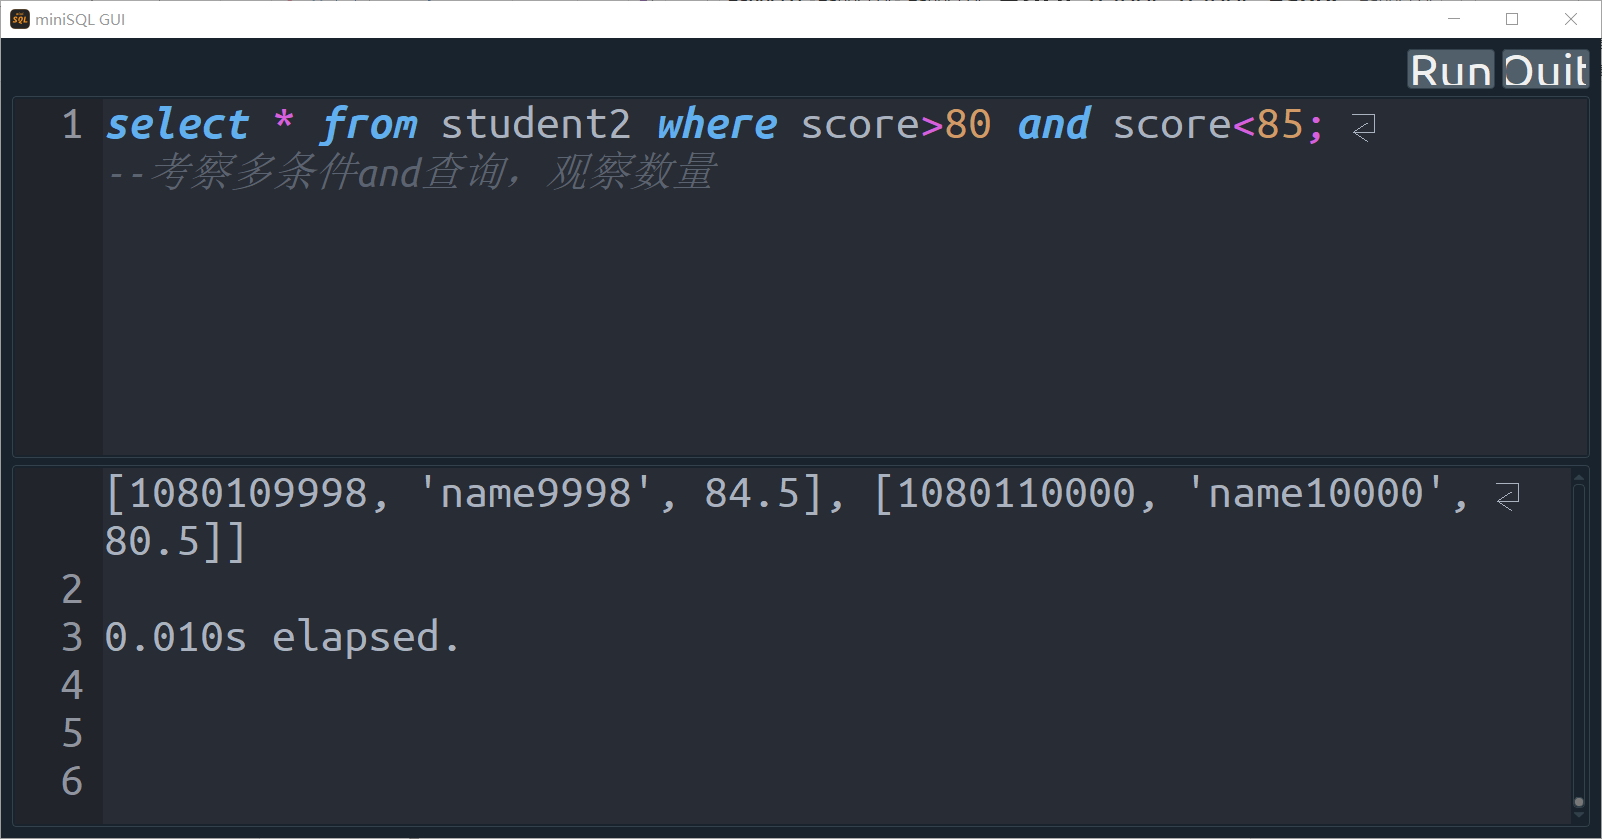
\includegraphics[width=0.8\linewidth]{figure/5.7.png}
    \caption{select-and}
    \label{fig:runtime5.7}
\end{figure}
\begin{figure}[H]
    \centering
    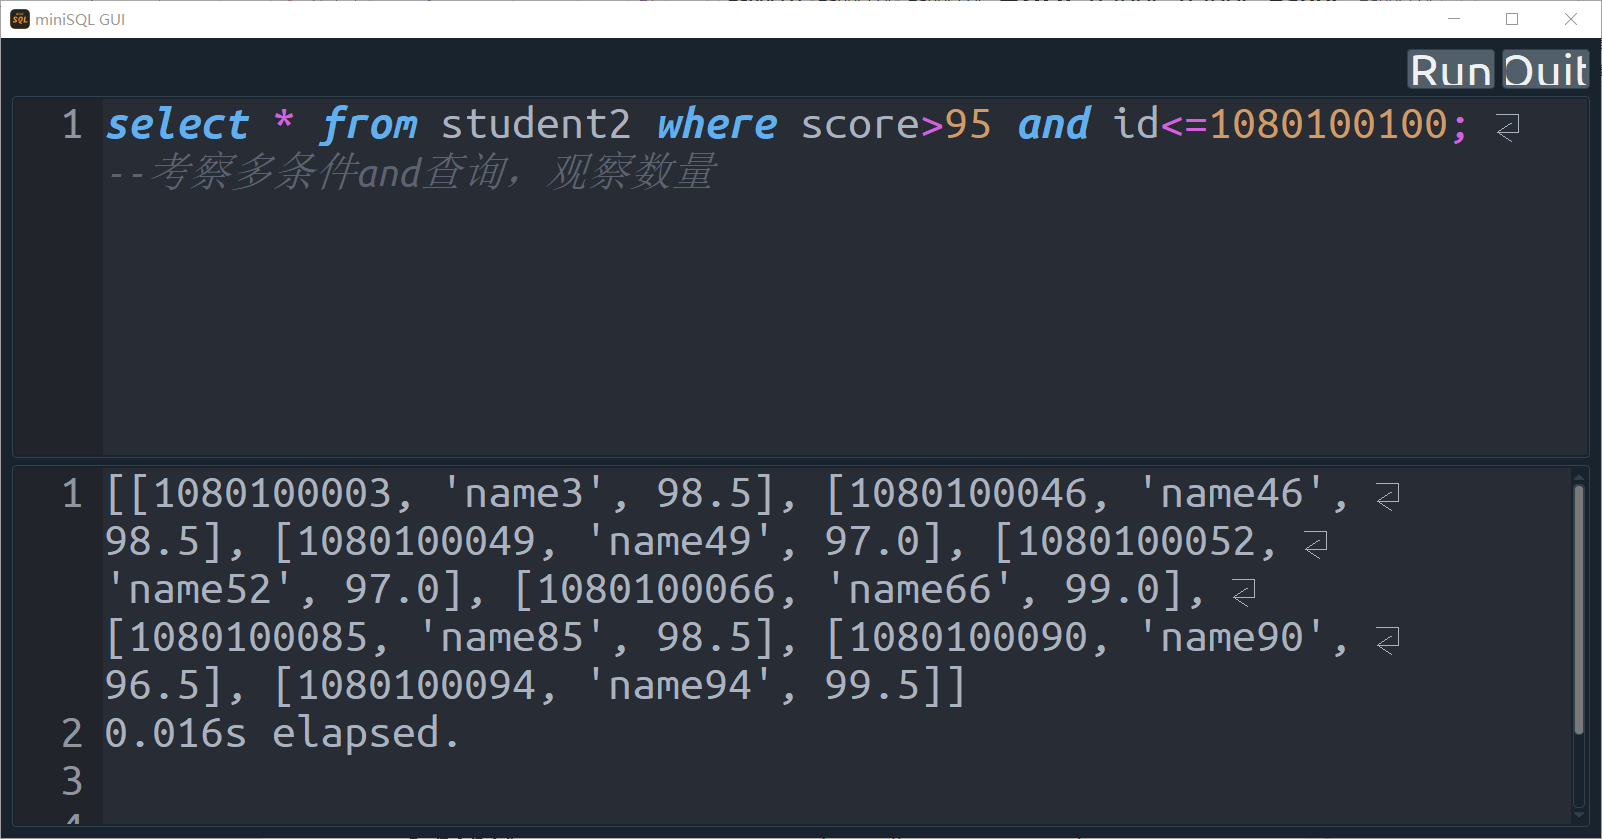
\includegraphics[width=0.8\linewidth]{figure/5.8.png}
    \caption{select-and}
    \label{fig:runtime5.8}
\end{figure}
\section{插入记录语句}
\subsection{执行流程}
1.GUI读入,调用API;
\par
2.API调用interpreter解析并处理错误;
\par
3.返回API,调用catalog manager得到unique并进行检查,得到index id并调用index manager进行insert (将调用buffer manager);
\par
4. 调用record manager进行insert(将调用buffer并可能调用file manager存取数据);
\par
5.API统计执行时间,返回给GUI输出。
\subsection{运行截图}
\begin{figure}[H]
    \centering
    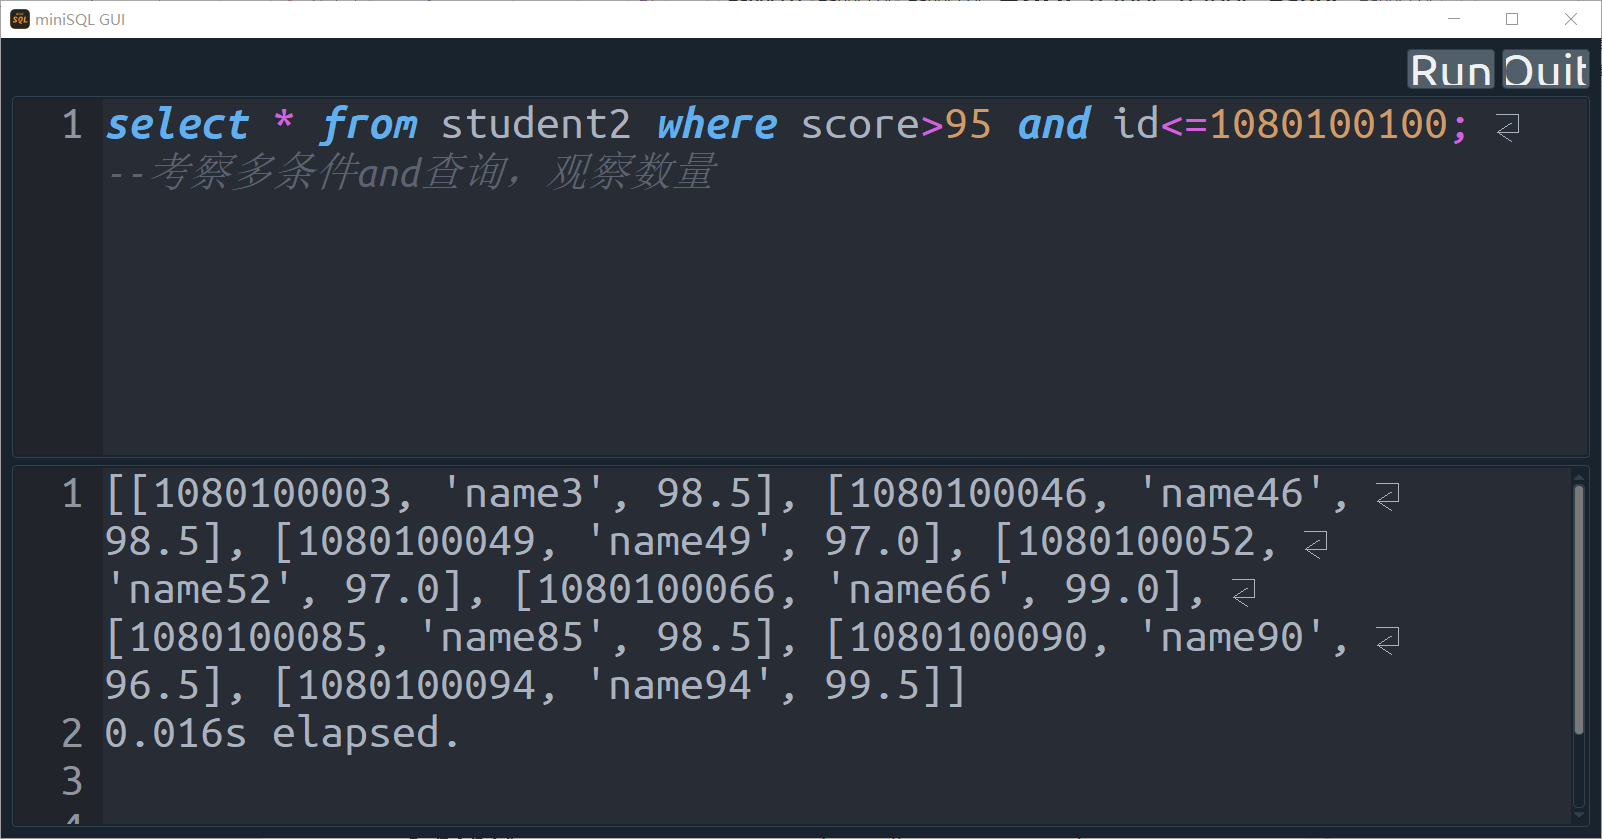
\includegraphics[width=0.8\linewidth]{figure/6.1.png}
    \caption{insert-failed}
    \label{fig:runtime6.1}
\end{figure}
\begin{figure}[H]
    \centering
    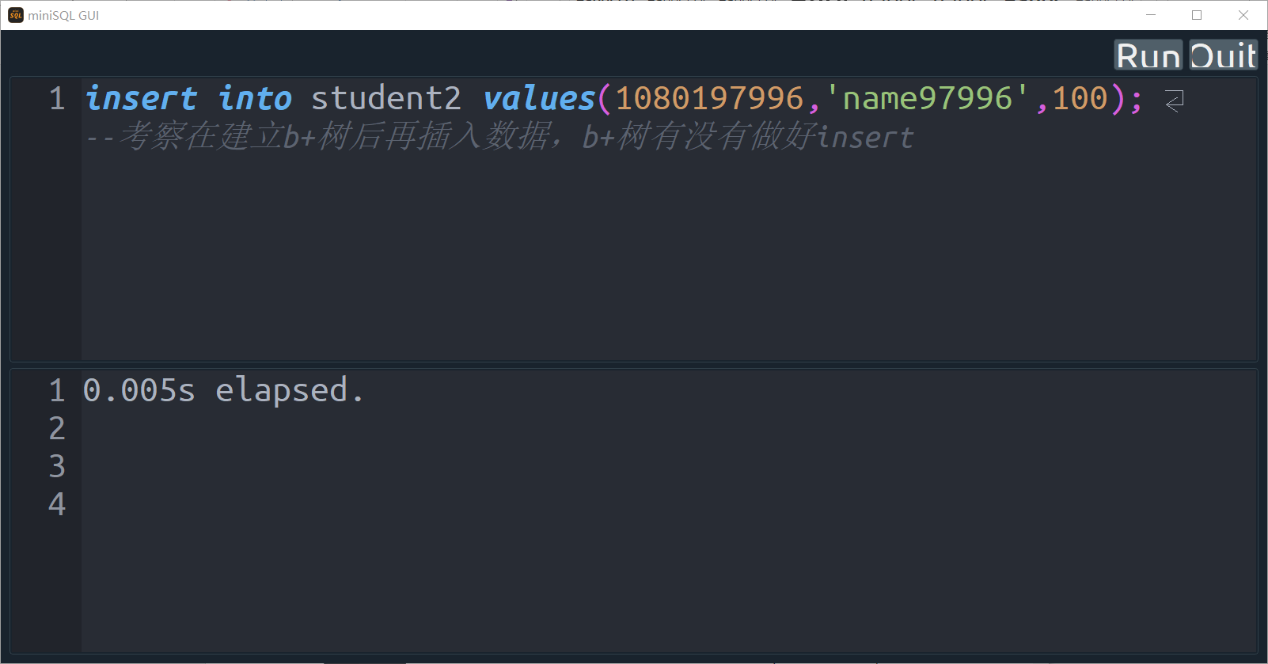
\includegraphics[width=0.8\linewidth]{figure/6.2.png}
    \caption{insert-succeed}
    \label{fig:runtime6.2}
\end{figure}
\section{删除记录语句}
\subsection{执行流程}
1.GUI读入,调用API;
\par
2.API调用interpreter解析并处理错误;
\par
3.返回API,调用catalog manager得到index id并调用index manager对对应index的数据进行删除(将用到buffer manager),调用record manager进行删除(将用到buffer manager并可能调用file manager进行文件读写);
\par
4.API统计执行时间,返回给GUI输出。
\subsection{运行截图}
\begin{figure}[H]
    \centering
    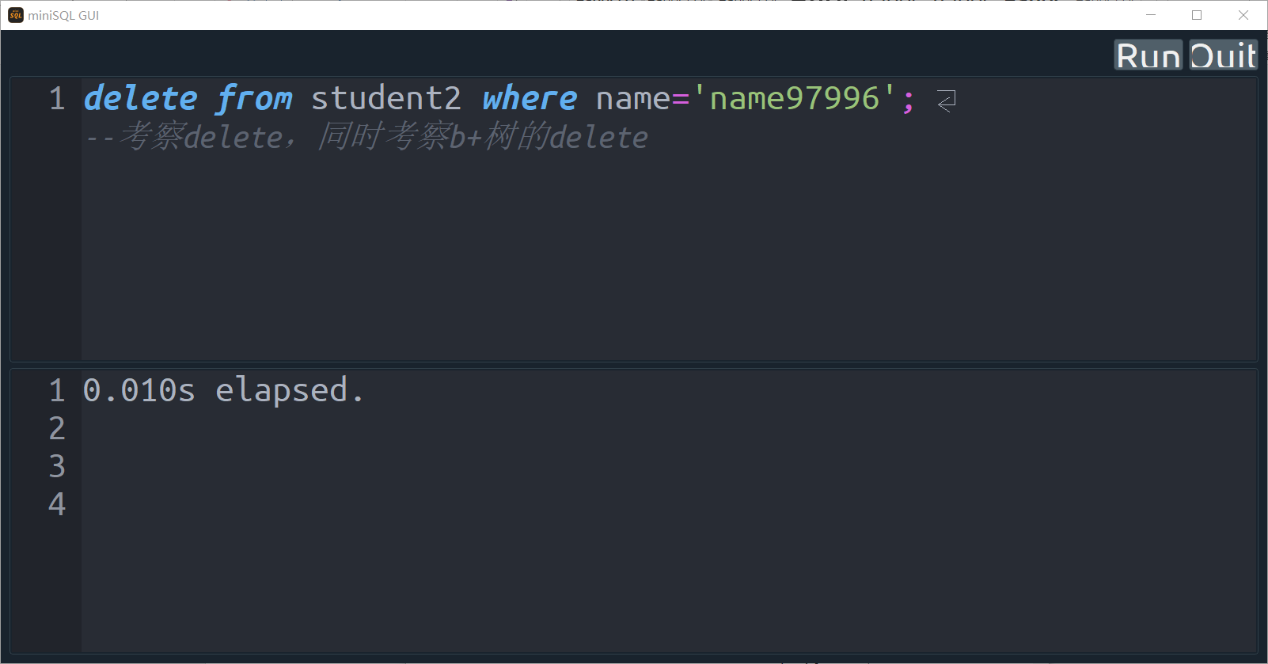
\includegraphics[width=0.8\linewidth]{figure/7.1.png}
    \caption{delete-use name(index)}
    \label{fig:runtime7.1}
\end{figure}
\begin{figure}[H]
    \centering
    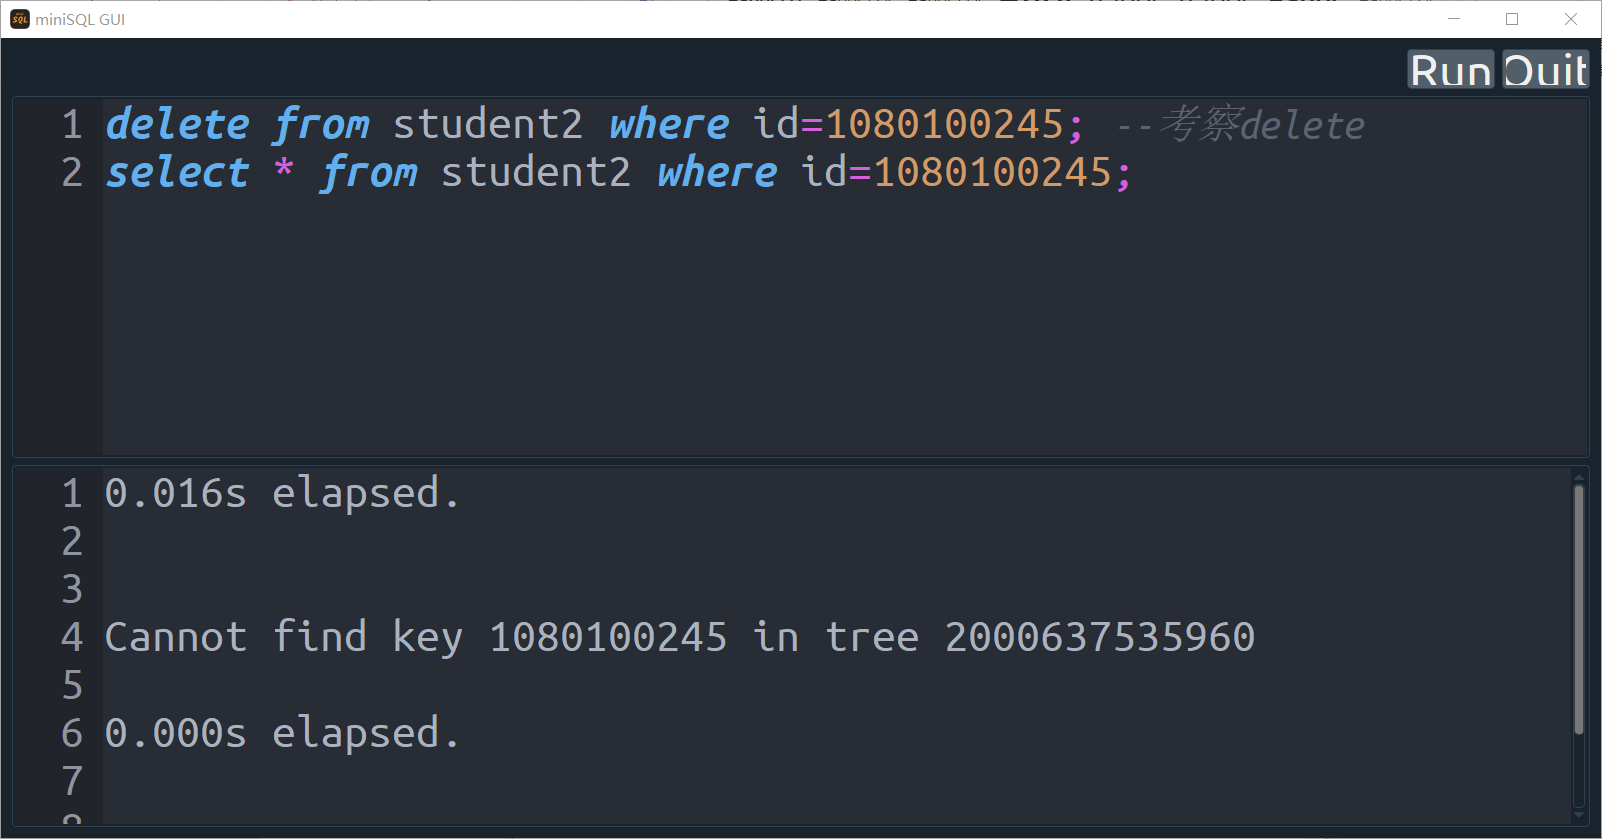
\includegraphics[width=0.8\linewidth]{figure/7.2.png}
    \caption{delete-use primary key}
    \label{fig:runtime7.2}
\end{figure}
\begin{figure}[H]
    \centering
    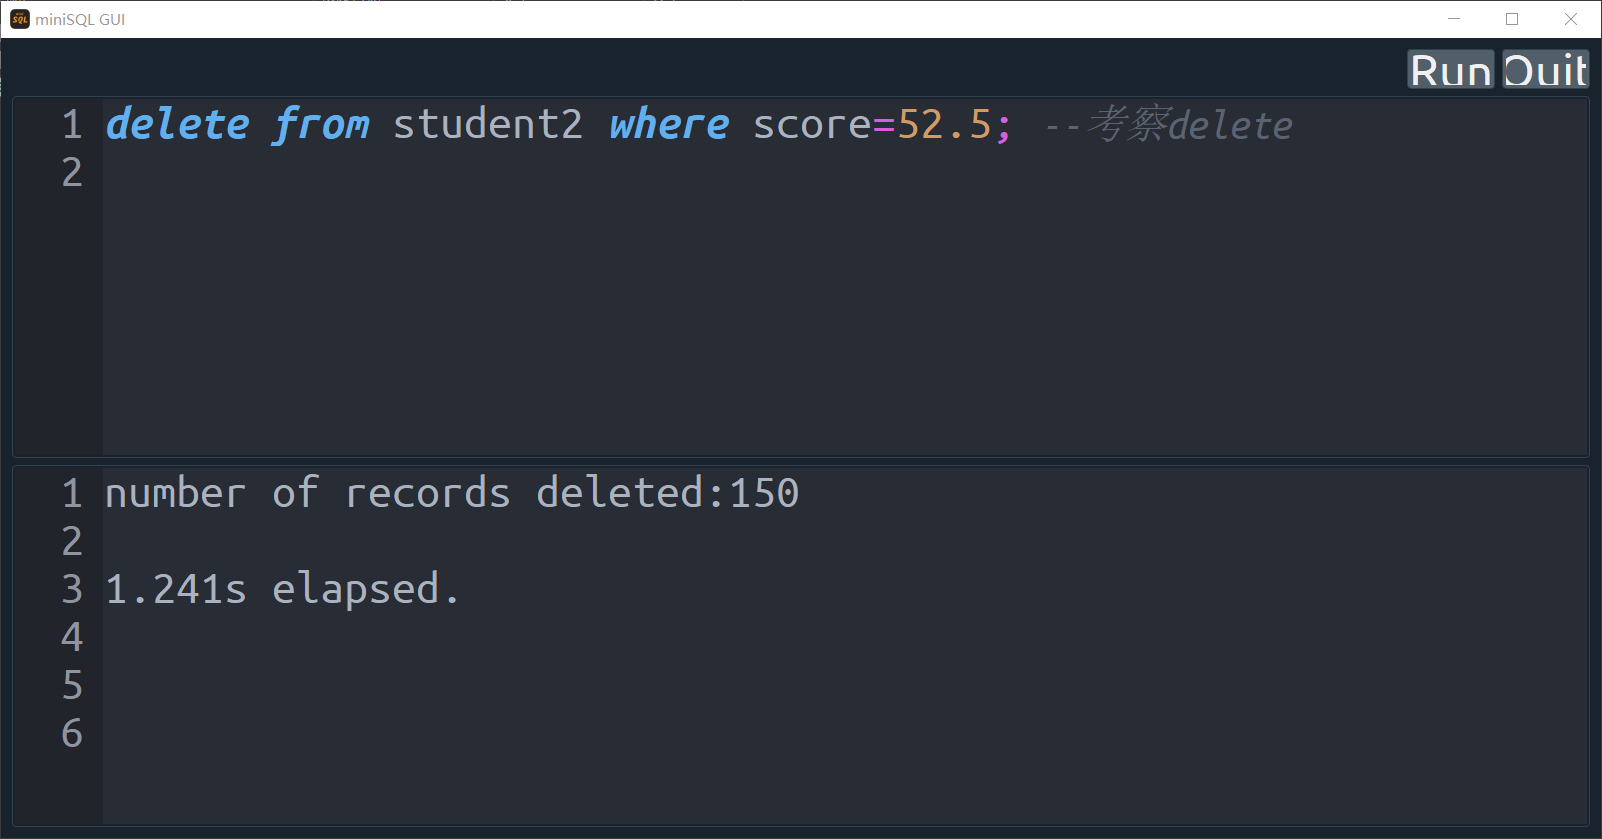
\includegraphics[width=0.8\linewidth]{figure/7.3.png}
    \caption{delete-use score}
    \label{fig:runtime7.3}
\end{figure}
\section{退出系统语句}
可以通过“quit;”语句和GUI界面中的quit按钮进行。
\par
退出时调用buffer manager->file manager将data,catalog和index的数据都存入文件。
\section{执行脚本文件语句}
\subsection{执行流程}
1.GUI读入,调用API;
\par
2.API调用interpreter解析并处理错误;
\par
3.返回API,读文件,将文件中读到的指令传给API中相应处理函数;
\par
4.API统计执行时间,返回给GUI输出并输出“one file done”。
\subsection{运行截图}
\begin{figure}[H]
    \centering
    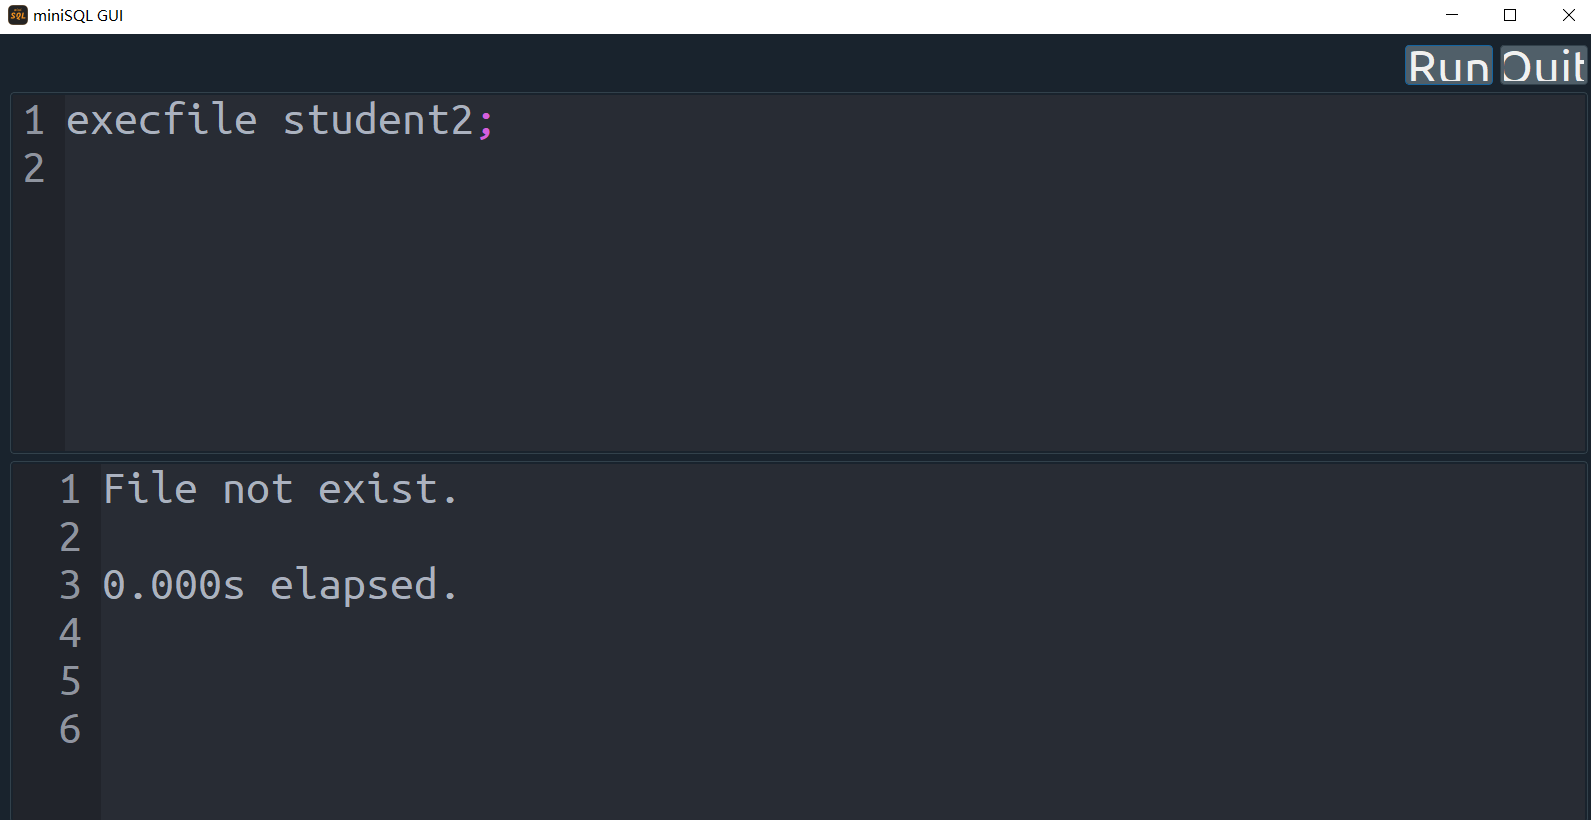
\includegraphics[width=0.8\linewidth]{figure/8.1.png}
    \caption{execfile-failed}
    \label{fig:runtime8.1}
\end{figure}
\begin{figure}[H]
    \centering
    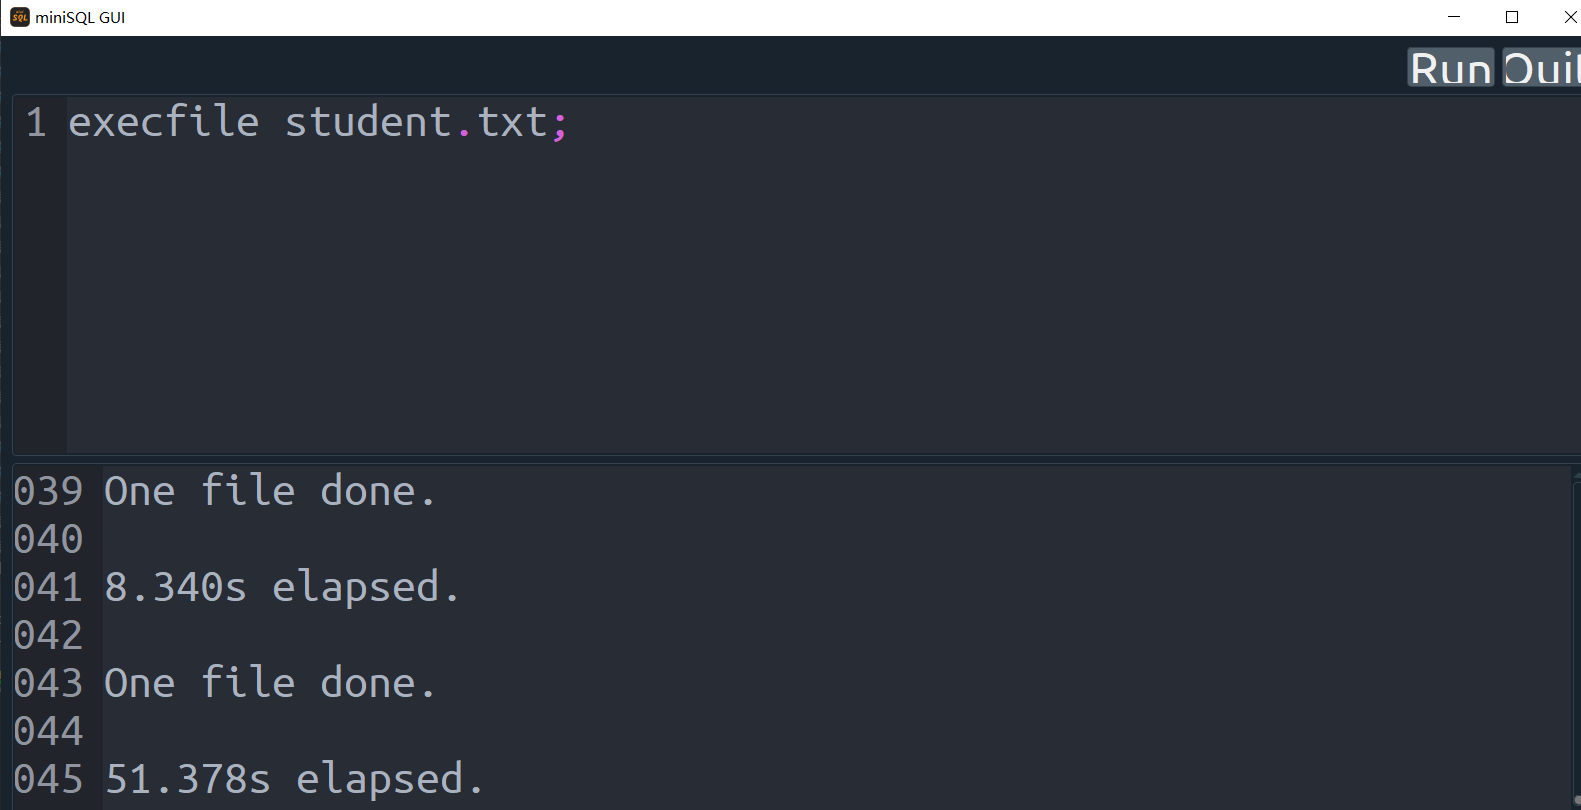
\includegraphics[width=0.8\linewidth]{figure/8.2.png}
    \caption{execfile-succeed}
    \label{fig:runtime8.2}
\end{figure}
\section{show语句}
\subsection{执行流程}
1.GUI读入,调用API;
\par
2.API调用interpreter解析并处理错误;
\par
3.返回API,调用catalog manager对需要显示的信息进行查询;
\par
4.API统计执行时间,返回给GUI输出。
\subsection{运行截图}
\begin{figure}[H]
    \centering
    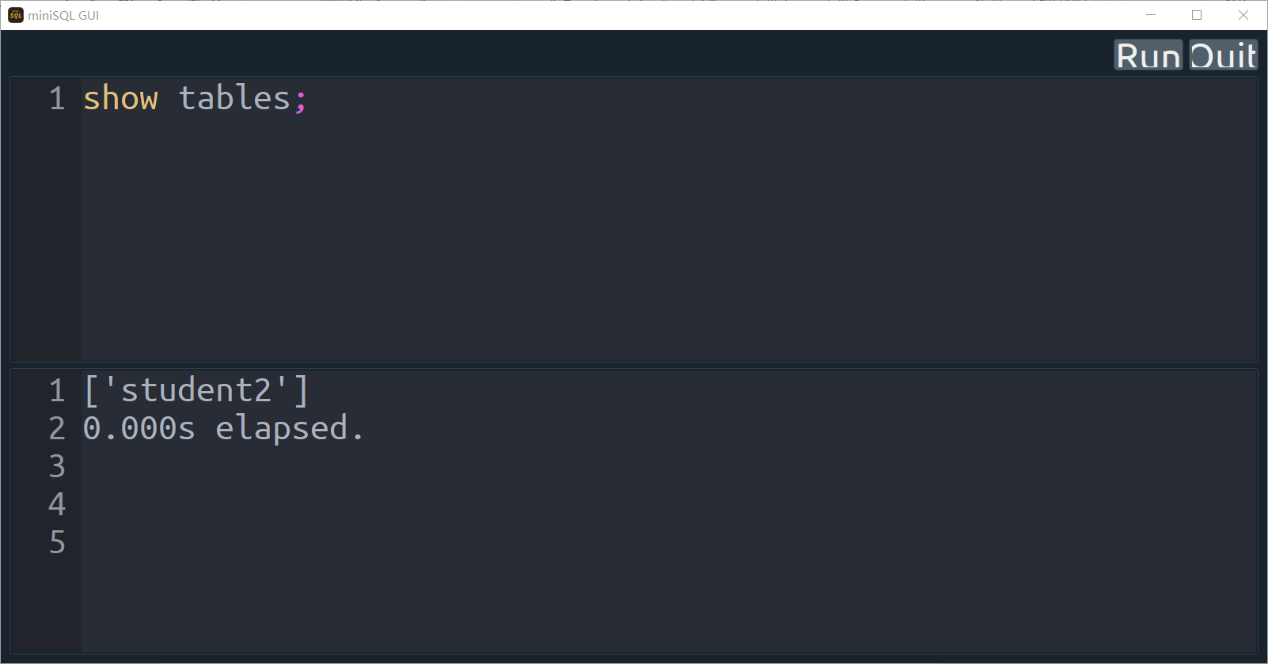
\includegraphics[width=0.8\linewidth]{figure/9.1.png}
    \caption{show tables}
    \label{fig:runtime9.1}
\end{figure}
\begin{figure}[H]
    \centering
    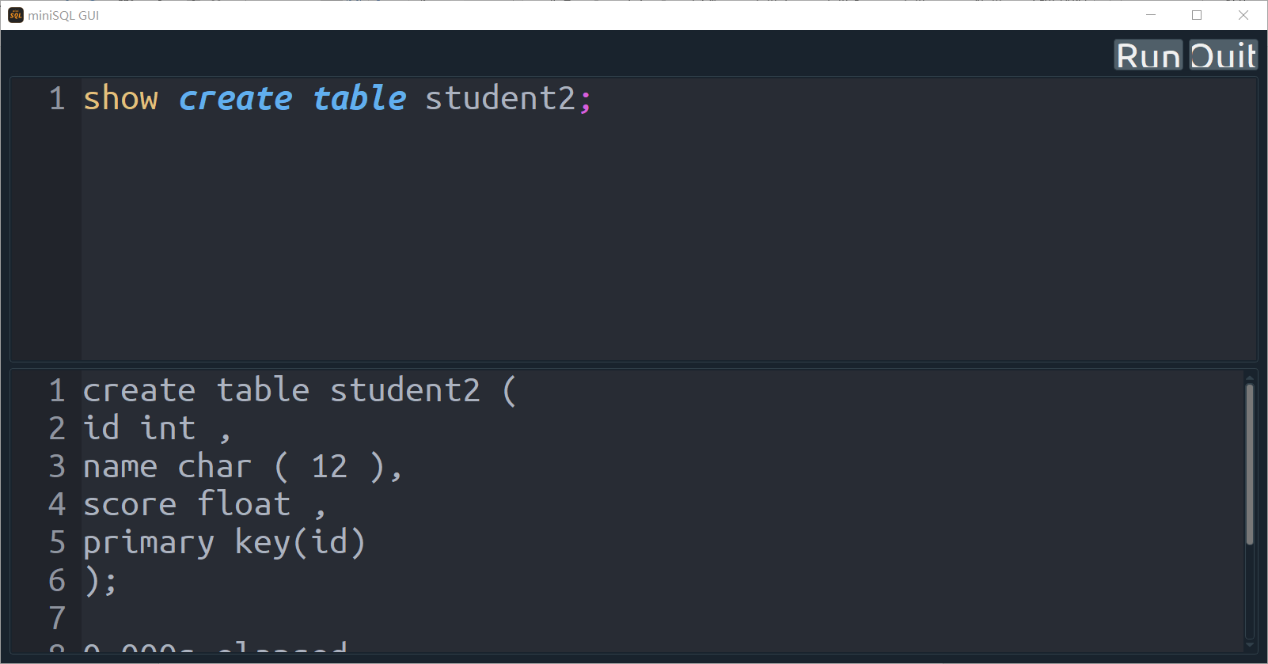
\includegraphics[width=0.8\linewidth]{figure/9.2.png}
    \caption{show create table}
    \label{fig:runtime9.2}
\end{figure}
\begin{figure}[H]
    \centering
    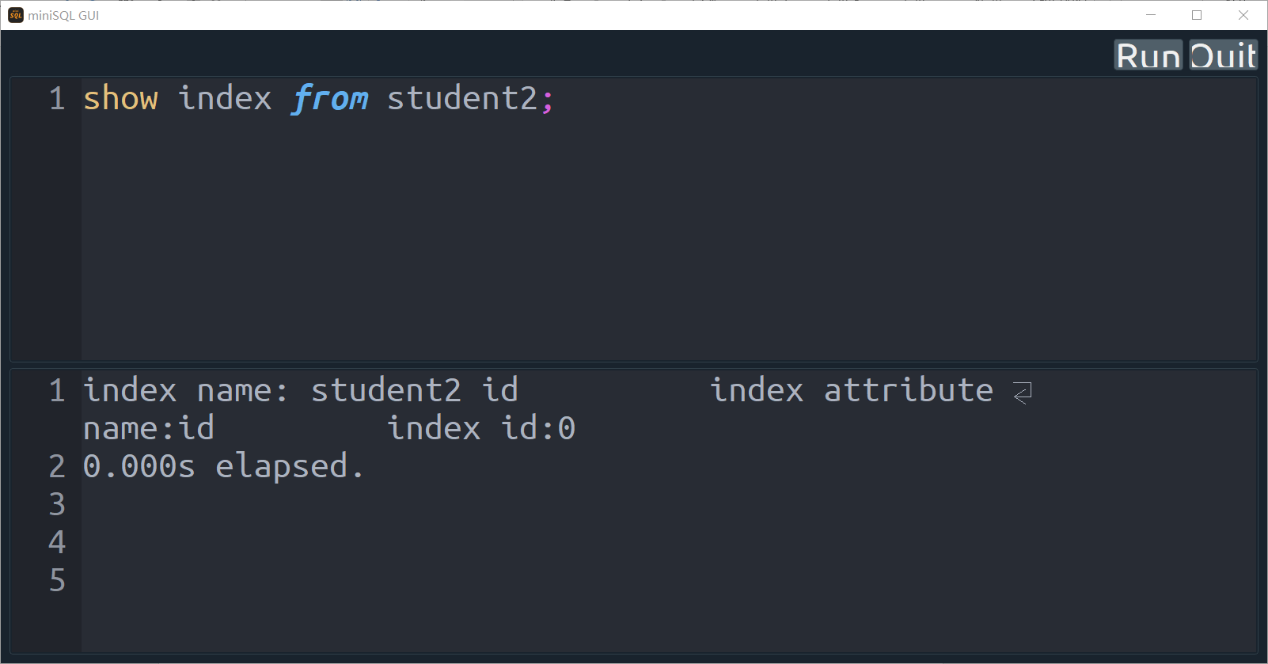
\includegraphics[width=0.8\linewidth]{figure/9.3.png}
    \caption{show index}
    \label{fig:runtime9.3}
\end{figure}

\chapter{总结}
\section{B+树,索引管理器与GUI}
在本实验中,我们从零实现了B+树模块。借助\texttt{Python}的动态类型语言特性,我们的B+树可以有效对各种\texttt{Python}支持的数据类型进行操作。通过进行单元测试,我们在miniSQL项目整体进行的前期就保证了B+树模块的正确性,为后续调试整合过程带来了极大方便。
\par
接着,我们实现了B+树中的索引相关操作。并封装成了一个易用的模块,使得API可以方便的调用。
\par
此次实验中我们深刻感受到了小组合作与提前定义接口的重要性,并且在B+树具体实现过程中,我们对单元测试的作用有了更进一步的了解。
\par
我们通过设计GUI进一步了解了程序设计过程中与人类交互方式的重要性。我们发现图形界面设计与命令行程序各有优劣,经过研究发现很多程序都采用命令行程序提供核心功能,接着通过图形界面将这些核心功能包裹。例如\texttt{Visual Studio}的\texttt{cl.exe}编译器
\section{API,interpreter与catalog manager}
在本实验中,我们实现了 API,catalog manager和interpreter模块。这三个模块是所有模块中难度相对较低,但是需要细、和耐心以及对minisql的实现流程和具体要求足够了解的部分。
\par
得益于小组另外两位成员的认真努力,调用封装好的record manager和index manager模块大大降低了API的实现难度。 但在完成过程中我们也遇到了很多问题,如果能够更好更仔细地交流好接口和类,这些问题其实能够更轻松解决。
\par
对于我个人来说,这是第一次通过git与小组成员合作完成代码,因为自己对这种合作模式的不熟悉给大家造成了不少麻烦;整个实验下来,最深的感受还是用更好的平台进行合作,确实能够方便小组交流合作,节省上传/下载/合并代码的时间。同时,在对minisql各种错误提示的处理中,也学到了利用python的exception和error类解决各种错误返回问题的方法,对如何写适用于可能状况百出的现实应用的代码有了基础的简单了解。
\section{record, buffer manager 与 DB Files}
在本实验中,我们实现了Record Manager,Buffer Manager,DB Files三个模块。这三个模块的关联性较大,难度适中,需要对数据库的内部有一定的理解,设计合适的存储形式并有耐心地一步步实现。
\par
此次实验中,我深刻体会到了小组讨论与合作中提前定义接口的重要性。一开始,我并不清楚应该从哪里入手,应该如何实现。幸运的是,在小组多次讨论后,终于有了一个比较清晰完整的实现思路。在小组成员的包容和帮助下,我最终实现了三个模块,并与小组成员实现的模块顺利对接接口。并在不断的打磨中尽量减少了bug。
\par
本次实验我们全程通过git来实现代码的共享和历史版本保存,方便了小组的线上实时交流合作,节约了时间,提高了效率。从数据库的知识角度看,我在对Buffer Manager的设计中更加深入理解了buffer在数据库数据查询/删除等操作中起到的作用,同时对行存储、列存储等多种形式存储方式有了一定的了解。从编程语言(python)角度看,我从几乎一窍不通到可以写一些代码,了解了python的基本类型和语法,理解了pickle,pandas等python包的强大之处。

\newpage
\part{附录}


\begin{appendices}
\chapter{接口说明}
\section{index}
\begin{longlisting}
    \begin{minted}{python}
def create_index(ind, data_list, cmp=dummy_cmp, is_primary=False):
    """
    :param ind: the id of the index to be saved to file
    :param data_list: the data, as list, to create index on
    :param cmp: the comparator of the index, defaults to operator<
    :param is_primary: whether we're dealing with primary key, using sorted list
    :return: index of the newly created table
    """


def drop_index(ind):
    """
    :param ind: the id of the index
    :return: currently nothing is returned
    """


def insert(ind, key, value, is_replace=False):
    """
    :param ind: the id of the index
    :param key: the key to insert into the index
    :param value: the value of the B+ tree, probably the line number of the inserted item
    :param is_replace: whether we should replace on duplication
    :raise KeyException: duplication
    """


def search(ind, key, is_greater=None, is_current=None, is_range=False, is_not_equal=False):
    """
    A thin wrapper around _operate
    :param is_current: whether we want a single value range search with current node
    :param is_greater: whether we want a single value range search of greater than
    :param ind: the id of the index to be deleted on
    :param key: the key/keys to be deleted (single or range)
    :param is_range: are we searching in range?
    :return: currently nothing is returned
    """


def delete(ind, key, is_greater=None, is_current=None, is_range=False, is_not_equal=False):
    """
    A thin wrapper around _operate
    :param is_current: whether we want a single value range search with current node
    :param is_greater: whether we want a single value range search of greater than
    :param ind: the id of the index to be searched on
    :param key: the key/keys to be searched (single or range)
    :return: currently nothing is returned
    """


def get_values(ind):
    """
    get every value from the bplus tree for printing all information fast enough
    :param ind: id of the index whose value is to be updated
    """


def update_values(ind, values):
    """
    updates information about an index
    :param ind: id of the index whose value is to be updated
    :param values: the new values to be set to the index
    :return:
    """
    \end{minted}
    \caption{接口说明}
    \label{lst:interface_specification}
\end{longlisting}

\section{API}
\begin{longlisting}
    \begin{minted}{python}
def command_prompt(file_file=None,str_command=None):
    """
    :param file_file: the file this function is expected to load and prompt
    :param str_command: the string this function is expected to load and prompt
    :return: if str_command is not None, return the string type running result
    """
    
def str_main(input):
    """
    :param input: string type instructions
    :return: string type running result of input instructions
    """
    
def main():
    """
    running in cmd and print the result
    """
    \end{minted}
    \caption{接口说明}
    \label{lst:interface_specification}
\end{longlisting}

\section{interpreter}
\begin{longlisting}
    \begin{minted}{python}
def translate(self, instruction):
    """
    :param instruction: string type instruction
    :return: dictionary type information of instruction or (class) error
    """
    \end{minted}
    \caption{接口说明}
    \label{lst:interface_specification}
\end{longlisting}

\section{catalog manager}
\begin{longlisting}
    \begin{minted}{python}
def check_table(self, name):
	"""
    :param name:string type name of table
    :return: 1 if the table exists, 0 otherwise
    """

def check_index(self, table_name, attribute_name):
    """
    :param table_name: string type name of table
    :param attribute_name: string type name of attribute
    :return: 1 if the attribute in this table has index, 0 otherwise
    """

def check_unique(self, table_name, attribute_name):
    """
    :param table_name: string type name of table
    :param attribute_name: string type name of attribute
    :return: 1 if the attribute in this table is unique, 0 otherwise
    """

def check_attribute(self, table_name, attribute_name):
    """
    :param table_name: string type name of table
    :param attribute_name: string type name of attribute
    :return: 1 if the attribute in this table exists, 0 otherwise
    """

def get_unique(self, table_name):
    """
    :param table_name: string type name of table
    :return: list of names of unique attributes in this table
    """

def get_index(self, table_name):
    """
    :param table_name: string type name of table
    :return: list of (class) index in this table
    """

def create_table(self, table, index):
    """
    create a new table in catalog
    :param table: (class) table
    :param table: (class) index of the primary key
    """

def create_index(self, index):
    """
    create a new index in catalog
    :param table: (class) index
    """

def drop_table(self, table_name):
    """
    drop a table in catalog
    :param table_name: string type name of table
    """

def drop_index(self, index_name):
    """
    drop a index in catalog
    :param index_name: string type name of index
    """

def check_index_name(self, index_name):
    """
    :param index_name: string type name of index
    :return: 1 if the index exists, 0 otherwise
    """

def get_attribute(self, table_name):
    """
    :param table_name: string type name of table
    :return: list of [name,type,length] of attributes in this table
    """

def get_primary(self, table_name):
    """
    :param table_name: string type name of table
    :return: name of key attribtue
    """

def get_index_attribute(self, table):
    """
    :param table_name: string type name of table
    :return: list of attribtue name of index in this table
    """

def get_index_info(self, index_name):
    """
    :param index_name: string type name of index
    :return: [table name, attribute name, index id] of the index
    """

def get_attribute_type(self, table_name, attr_name):
    """
    :param table_name: string type name of table
    :param attr_name: string type name of attribute
    :return: type of the attribute in this table
    """

def get_index_id(self, table_name, attribute_name):
    """
    :param table_name: string type name of table
    :param attribtue_name: string type name of attribute
    :return: index id of the index of the attribute in this table
    """

def get_attribute_cnt(self, table_name, attr_name):
    """
    :param table_name: string type name of table
    :param attr_name: string type name of attribute
    :return: number the arrtibutes from 1 to n, return the number of required arribute
    """

def get_all_table(self):
    """
    :return: list of table names in this database
    """
    \end{minted}
    \caption{接口说明}
    \label{lst:interface_specification}
\end{longlisting}

\section{record manager}
\begin{longlisting}
    \begin{minted}{python}
def insert_record(fname, record):
    """
    :param fname: the name of the table
    :param record: a tuple of a record
    :return: the insertion position of the record
    """
    
def delete_record_with_Index(fname, indList, conditionList):
    """
    delete one or a serial of records using or not using Index
    if use Index, the indList is a list, and the indList is 0 if not
    :param fname: the name of the table
    :param indList: the position of selected records from index manager
    :param conditionList: a list of objects of class Condition
    :return: the list of position of deleted records
    """

def select_record_with_Index(fname, indList, conditionList):
    """
    select one or a serial of records using or not using Index
    if use Index, the indList is a list, and the indList is 0 if not
    :param fname: the name of the table
    :param indList: the position of selected records from index manager
    :param conditionList: a list of objects of class Condition
    :return: the list of selected records  
    """

def create_table(fname):
    """
    :param fname: the name of the table
    """

def delete_table(fname):
    """
    :param fname: the name of the table
    """

def clear_table(fname):
    """
    :param fname: the name of the table
    """
    \end{minted}
    \caption{接口说明}
    \label{lst:interface_specification}
\end{longlisting}

\section{buffer manager}
\begin{longlisting}
    \begin{minted}{python}
def insert_record(self, tname, record):
    """
    :param tname: the name of the table
    :param record: a tuple of a record
    :return: the insertion position of the record
    """
    
def get_blocks(self, tname): 
    """
    :param tname: the name of the table
    :return: a list of all the blocks in the table
    """

def create_table(self, tname):
    """
    :param tname: the name of the table
    """

def delete_table(self, tname):
    """
    not only delete the table file, but also in buffer
    :param tname: the name of the table
    """

def clear_table(self, tname):
    """
    not only clear the table file, but also in buffer
    :param tname: the name of the table
    """

def get_index(Ind):
    """
    :param Ind: the serial number of a B+ tree
    :return: a B+ tree structure
    """
    
def save_index(tree, Ind):
    """
    :param tree: a B+ tree structure 
    :param Ind: the serial number of a B+ tree
    """
    
def delete_index(Ind):
    """
    :param Ind: the serial number of a B+ tree
    """
    
def initialize_buffer():
    """
    initialize the freeList, index_buffer, maxrecordNum(get datas from files)
    """
    
def quit_buffer():
    """
    save the freeList, index_buffer, maxrecordNum into files
    """

    \end{minted}
    \caption{接口说明}
    \label{lst:interface_specification}
\end{longlisting}

\section{DB Files}
\begin{longlisting}
    \begin{minted}{python}
def initialize_file():
    """
    if there is no Document Folders 'data', 'index', 'catalog', create them
    """

def insert_new_record(fname, record):
    """
    :param fname: the name of the table
    :param record: a tuple of a record
    """

def write_back(data_block):
    """
    write the content of the data_block back into the file, called when LRU happens
    :param data_block: an object of the class DataBlock
    """

def get_block_data(fname, blockpos):
    """
    :param fname: the name of the table
    :param blockpos: the position of the certain block in the file
    :return: the content of one block in the file at the position of blockpos
    """

def create_data_file(fname):
    """
    create a file of a table
    :param fname: the name of the table
    """
    
def delete_data_file(fname):
    """
    delete the file of a table
    :param fname: the name of the table    
    """

def clear_data_file(fname):
    """
    clear the file of a table
    :param fname: the name of the table    
    """
    
def save_index_file(index_buffer):
    """
    :param index_buffer: buffer of index in buffer manager
    """
    
def get_index_file():
    """
    get the index_buffer from file when initializing
    :return: the index_buffer
    """

def save_catalog_file(catalogManager):
    """
    :param catalogManager: catalog(contain the metadata) in catalog manager
    """

def get_catalog_file():
    """
    get the metadata for catalog manager from file when initializing
    :return: the catalog(contain the metadata)   
    """

def save_freeList(freeList):
    """
    :param freeList: freeList in buffer manager to save
    """
    
def get_freeList():
    """
    get the freeList for buffer manager from file when initializing
    :return: the freeList
    """

def save_maxrecordNum(maxrecordNum):
    """
    :param maxrecordNum: freeList in buffer manager to save
    """

def get_maxrecordNum():
    """
    get the maxrecordNum for buffer manager from file when initializing
    :return: the maxrecordNum
    """
    \end{minted}
    \caption{接口说明}
    \label{lst:interface_specification}
\end{longlisting}

\chapter{插图,表格与列表}
\listoffigures
% \listoftables
\listoflistings
\end{appendices}
\end{document}